% !TeX root = main.tex
\section*{Empfohlene Literatur}

\fullcite{MacKay03InformationTheory} (sehr ausführlich und anschaulich; mathematisch teilweise unsauber)

\fullcite{Ash90InformationTheory} (Standardwerk)

\fullcite{Willems08CodKrypt}

\fullcite{KerstingWakolbinger08Stoch} (Sehr gutes deutsches Buch zur Stochastik mit einem kurzen Kapitel zur Informationstheorie)


\section*{Einführung}
Die heutige Zeit ist durch die Allgegenwart \emph{digitaler Information} und deren Verbreitung bzw.\ Verarbeitung geprägt. Zur Informationsübertragung werden verschiedene Medien wie Telefon- und Netzwerkkabel, die Luft (Mobilfunk, Radio, DVB-T), der Weltraum (Satellitenkommunikation), aber auch DVDs oder USB-Sticks genutzt.

All diesen \emph{Kommunikationskanälen} (den Ausdruck werden wir später präzise definieren) ist gemein, dass sie von unausweichlichem Rauschen bei der Datenübertragung betroffen sind; sei es aufgrund von Umwelteinflüssen auf dem Übertragungskanal (elektromagnetische Störungen, Wettereffekte, Kratzer, \dots) oder technische Unzulänglichkeiten der beteiligten Elektronik (Qualität der sendenden / empfangenden Antennen, Schaltkreise zur Signalverarbeitung, etc.). Die meisten Anwendungen setzen jedoch eine praktisch fehlerfreie Übertragung voraus; lädt man etwa ein Computerprogramm herunter, kann schon ein einziges fehlerhaftes Bit dafür sorgen, dass das Programm nicht funktioniert.

Die \emph{Informationstheorie} beschäftigt sich daher mit der Analyse von Kommunikationssystemen, die man schematisch wie folgt darstellen kann:
\begin{Center}
  \begin{tikzpicture}
    \node[box=source]  (source)                    {Datenquelle};
    \node[box=encoder] (encoder) [right=of source] {Codierer} edge[<-] (source);
    \node[box=channel] (channel) [right=of encoder] {Kanal} edge[<-] (encoder);
    \node[box=encoder] (decoder) [right=of channel] {Decodierer} edge[<-] (channel);
    \node[box=source] (receiver) [right=of decoder] {Empfänger} edge[<-] (decoder);
    \node[box=channel] (noise) [above=of channel] {Rauschen} edge[->] (channel);
   \end{tikzpicture}
\end{Center}
Die Datenquelle besteht aus einer Person oder einer Maschine, welche die zu übertragende Information produziert. Der Codierer hat die Aufgabe, diese Nachricht in eine Form zu übersetzen, die zur Übertragung auf dem Kanal geeignet ist. Dies kann je nach Anwendung \zB eine Folge von Bits oder auch ein elektromagnetisches Signal sein. Außerdem soll die codierte Nachricht robust gegen die durch das Kanalrauschen eintretenden Übertragungsfehler sein; der Codierer muss also irgendeine Form von \emph{Redundanz} einbauen, so dass der \emph{Decodierer} Fehler erkennen oder sogar korrigieren kann. Allerdings reduziert diese Redundanz die nutzbare Übertragungsrate des Kanals, so dass wir es mit zwei entgegengesetzten Zielen – niedrige Fehlerrate, aber hohe Übertragungsrate – zu tun haben.

%Das wichtigste Resultat der Informationstheorie besagt, dass man durch geeignete Codierung über einen verrauschten Kanal Information mit beliebig kleiner Fehlerwahrscheinlichkeit senden kann, solange die Codierungsrate unter der \emph{Kapazität} des Kanals liegt. Die genaue Bedeutung der Begriffe \emph{Information}, \emph{Kanal}, \emph{verrauscht}, \emph{Codierungsrate} und \emph{Kapazität} wird dabei im Lauf der Vorlesung präzisiert. Das folgende Beispiel erlaubt jedoch bereits einen Intuitiven Blick auf die Bedeutung des obigen Resultats.

\begin{example}\label{ex:codingIntro}
  Eine Datenquelle produziere fortlaufend Bits, also Buchstaben aus dem Alphabet $\GF(2) = \{0,1\}$, mit der Rate \SI{1}{\bit\per\second}. Die Werte $0$ und $1$ sollen dabei mit gleicher Wahrscheinlichkeit auftreten und die einzelnen Bits unabhängig voneinander verteilt sein, so dass die Quelle dem wiederholten Werfen einer perfekten Münze entspricht. Die Bits werden über einen ebenfalls binären Kanal übertragen, der höchstens einmal pro Sekunde in Anspruch genommen werden kann, der jedoch mit Wahrscheinlichkeit $ε=\frac14$ ein Bit falsch überträgt, also aus der $0$ eine $1$ macht oder umgekehrt (auch der Kanal soll aufeinanderfolgende Übertragungen unabhängig voneinander beeinflussen).
  
  Ist nun die Fehlerrate von $ε=\frac14$ für unsere Zwecke zu hoch (in der Praxis sind oft Garantien in der Größenordnung $ε< 10^{-15}$ gefordert), müssen wir die Zuverlässigkeit des Systems erhöhen. Die einfachste Möglichkeit ist, jedes von der Quelle emittierte Bit mehrmals, \zB dreimal, zu senden. Der Codierer besteht dann aus der Funktion $E\colon \GF(2) → \GF(2)^3$, $E(a) = aaa$. Der Decodierer führt für jedes empfangene Tripel eine \enquote{Mehrheitsentscheidung} durch, decodiert es also genau dann als $1$, wenn es mindestens zwei Einser enthält:
  \begin{align*}
    &D\colon \GF(2)^3 → \GF(2)\\
    &D(a_1a_2a_3)= \begin{cases}
      0\tk   &\text{falls  }\abs{\{i\in\{1,2,3\}\colon a_i = 0\}} ≥ 2\\
      1      &\text{sonst.}
      \end{cases}
  \end{align*} Solange der Kanal höchstens eines der drei Bits verfälscht, kann der Decodierer so das gesendete Bit korrekt rekonstruieren; andernfalls ($2$ oder $3$ Fehler) liegt er falsch.
  
  Die \emph{Bit-Fehlerwahrscheinlichkeit}, also die Wahrscheinlichkeit, dass ein gesendetes Nutzdaten-Bit beim Empfänger (nach dem Decodieren) falsch ankommt, liegt damit bei 
  \[ P(2\text{ oder }3\text{ Fehler}) = \binom32 \(\frac14\)^2 \frac34 + \binom33 \(\frac14\)^3 \( \frac34\)^0 = \frac{10}{64} ≈ 0{,}16 < \frac14.\]
  Wir haben also die Fehlerwahrscheinlichkeit reduziert; der Preis dafür ist allerdings, das wir die Quelle auf \SI{1/3}{\bit\per\second} drosseln müssen, da der Kanal ja nur \SI{1}{\bit\per\second} annimmt – anders gesagt, pro Kanal-Bit wird im Schnitt nur noch $1/3$ Nutzdaten-Bit übertragen. Das Verhältnis von Quell-Bitrate zu Kanal-Bitrate wird \emphex{Codierungsrate} oder einfach \emphex{Rate} des Systems genannt.
\end{example}

\begin{exercise}\label{ex:repetitionCode}
Verallgemeinern Sie das Verfahren aus \cref{ex:codingIntro} auf beliebige Fehlerwahrscheinlichkeit des Kanals $ε<\frac12$ und $n$-fache Bitwiederholung für ungerade $n$. Zeigen Sie: Mit wachsendem $n$ geht zwar die Wahrscheinlichkeit eines Decodierfehlers gegen $0$, die Rate allerdings auch.
\end{exercise}

Die Informationstheorie geht der Frage nach, was hier überhaupt theoretisch erreichbar ist: Wie klein muss die Rate werden, um eine bestimmte, noch akzeptable Fehlerwahrscheinlichkeit erreichen zu können? Das wichtigste Resultat besagt, dass es (anders als beim Verfahren in \cref{ex:repetitionCode}) zum Erreichen einer beliebig kleinen Fehlerwahrscheinlichkeit \emph{nicht} notwendig ist, die Rate bis auf $0$ zu reduzieren: solange die Rate unterhalb der \emph{Kapazität} des Kanals liegt (die wir später noch definieren werden), können wir die Fehlerwahrscheinlichkeit durch geeignete Codierungsverfahren beliebig reduzieren, \emph{ohne die Rate weiter zu senken}. Im ersten Kapitel dieser Vorlesungshälfte (\cref{chap:IT}) werden wir dieses Resultat formalisieren und beweisen. Da der Beweis leider nicht konstruktiv ist, geht es danach in der \emph{Codierungstheorie} (\cref{chap:cod}) um konkrete Codierungsverfahren, die diese Kapazität zu erreichen versuchen.

Zunächst werden wir allerdings von einem fehlerfreien Kanal ausgehen und untersuchen, wie wir seine Übertragungsrate durch Codierung der Nachrichten möglichst effizient ausnutzen können. Denken wir beim Kanal an ein digitales Speichermedium, entspricht das der äquivalenten Frage, wie man die Daten aus der Quelle mit möglichst geringem Speicherverbrauch codieren kann (\emph{Datenkompression}). Dabei begegnen wir dem Begriff der \emph{Entropie} oder \emph{mittleren Ungewissheit} einer Nachrichtenquelle und werden sehen, dass die Entropie mit der optimal erreichbaren Kompression zusammenhängt.

\chapter{Informationstheorie}\label{chap:IT}
\section{Kommunikation über fehlerfreie Kanäle / Datenkompression}\label{chap:sourceCoding}
Wir gehen in diesem Kapitel von einer fehlerfreien Übertragung ohne Rauschen aus:
\begin{Center}
  \begin{tikzpicture}
    \node[box=source]  (source)                    {Datenquelle};
    \node[box=encoder] (encoder) [right=of source] {Codierer} edge[<-] (source);
    \node[box=channel] (channel) [right=of encoder] {Kanal} edge[<-] (encoder);
    \node[box=encoder] (decoder) [right=of channel] {Decodierer} edge[<-] (channel);
    \node[box=source] (receiver) [right=of decoder] {Empfänger} edge[<-] (decoder);
   \end{tikzpicture}
\end{Center}
Der Kanal gebe beim Empfänger also immer genau das aus, was beim Sender eingegeben wurde. Der Einfachheit halber beschränken wir uns auf einen \emph{binären} Kanal, der Bits (Buchstaben von $\GF(2)$) überträgt. Da es keine Übertragungsfehler zu berücksichtigen gibt, bleibt von den in der Einführung formulierten Zielen nur noch die möglichst hohe Übertragungsrate übrig. Wir gehen also folgender Frage nach:
\begin{question}\label{q:sourceCoding}
  Wie kann ein Codierer die Daten aus der Datenquelle möglichst sparsam zu binären Nachrichten codieren, wobei gewährleistet bleiben muss, dass der Decodierer die Daten wieder eindeutig rekonstruieren kann?
  
  Stellt man sich unter dem (abstrakten) Kanal ein Speichergerät vor, haben wir die äquivalente Frage, wie man gegebene Daten mit möglichst geringem Speicherverbrauch abspeichern kann.
\end{question}

Dazu formalisieren wir zunächst den Begriff der Quelle, die nichts weiter ist als eine Zufallsvariable.
\begin{definition}[Quelle]
  Eine \emph{(Daten-)quelle}\index{Quelle}\index{Datenquelle} $(A, X)$ besteht aus einem Alphabet $A=\{a_1,\dotsc,a_s\}$, $s=\abs A$ und einer Zufallsvariable $X$ mit Zielbereich $A$, welche die Wahrscheinlichkeit eines einzelnen Buchstabens \[p_i \coloneqq P_X(a_i) = P(X=a_i)\]
  der Quelle angibt. Die Buchstaben werden auch \emph{Symbole} oder \emph{Nachrichten} genannt, die Zufallsvariable $X$ nennen wir einen \emph{zufälligen Buchstaben}.
  
  Wir nehmen durchweg an, dass die Quelle beliebig viele Buchstaben generieren kann, die alle unabhängig voneinander nach $P_X$ verteilt sind. Die $N$-dimensionale Zufallsvariable $X^N$ ist dann ein \emph{zufälliges $N$-Wort} aus der Quelle, mit $P_{X^N}(x_1\dotsm x_N) = \prod_{i=1}^N P_X(x_i)$.
\end{definition}
\begin{remark}
  In der Schule oder auch in der Stochastik-Vorlesungen werden Wahrscheinlichkeiten oft benutzt, um die relative Häufigkeit eines beliebig oft wiederholbaren Experiments (beispielsweise des Werfens einer Münze) zu beschreiben. In unserem Kontext ist es hilfreich, sich die Wahrscheinlichkeit viel allgemeiner als ein Maß dafür vorzustellen, wie sicher bzw.\ unsicher man sich darin ist, dass ein bestimmtes Ereignis eintritt. Dieses ist unweigerlich subjektiv: schickt etwa eine Person $A$ eine SMS mit dem Endstand seines Fußballspiels an $B$, so ist deren Inhalt natürlich nicht zufällig, sondern eindeutig durch das bereits stattgefundene Spiel determiniert. Aus Sicht von $B$, der das Spiel nicht gesehen hat, kann der Spielstand vor Eintreffen der Nachricht aber durchaus durch eine Zufallsvariable modelliert werden, in deren Verteilung \zB seine Einschätzung der Spielstärken beider Mannschaften einfließen können.
\end{remark}

\subsection{Kompaktkurs Stochastik \RN{2}}
Wir wiederholen einige weitere stochastische Grundlagen.

\begin{definition}[Erwartungswert und Varianz]
  Der \emphex{Erwartungswert} einer reellen Zufallsvariable $X$ mit Alphabet $A=\{a_1,\dotsc, a_s\}$ ist definiert als
  \[ μ_X = \E[X] = \sum_{i=1}^s a_i P(X=a_i) = \sum_{i=1}^s a_i p_i. \]
  Als ihre \emphex{Varianz} bezeichnet man die erwartete quadratische Abweichung vom Mittelwert:
  \[ σ^2_X = \E[(X-\E[X])^2]\]
\end{definition}

\begin{theorem}[Schwaches Gesetz der großen Zahlen]\label{thm:lln}\index{Gesetz der großen Zahlen (schwaches)}
  Seien $X_1, \dotsc, X_N$ unabhängige Zufallsvariablen, alle mit dem gleichen Erwartungswert $μ=μ_{X_i}$ und Varianz $σ^2 = σ^2_{X_i}$. Sei $\bar X_N = \frac1N \sum_{n=1}^N X_n$ der Stichproben-Mittelwert von $X_1,\dotsc, X_N$. Dann gilt:
  \[ P\((\bar X_N - μ)^2 ≥ α \) ≤ \frac{σ^2}{αN}\]
  für alle $α > 0$: $\bar X_N$ nähert sich $μ$ mit wachsendem $N$ immer mehr an.
\end{theorem}
\begin{figure}
  \centering
  \begin{tikzpicture}[node distance=2cm and 5cm]
    \node (om) {$Ω$};
    \node [right=of om] (a) {$A$} edge[<-,"$X$" above] (om);
    \node [below=of a] {$A'$} edge[<-,"$h$" right] (a)
                              edge[<-,"$h(X)$" below] (om);
  \end{tikzpicture}
  \caption{Verkettung der Zufallsvariable $X$ mit einer Abbildung $h$ zur neuen Zufallsvariable $h(X)$ (\cref{rem:rvChaining}).}
  \label{fig:rvChaining}
\end{figure}
\begin{remark}\label{rem:rvChaining}
  Sei $Ω$ ein Wahrscheinlichkeitsraum und $X\colon Ω→A$ eine Zufallsvariable. Ist $h\colon A→A'$ eine Abbildung von $A$ in eine Menge $A'$, wird die Verkettung $h∘X$ zu einer neuen Zufallsvariablen mit Zielbereich $A'$, die wir mit $h(X)$ notieren (\cref{fig:rvChaining}). Ihre Verteilung ist gegeben durch
  \[ P_{h(X)}(S') = P(h(X) ∈ S') = P(ω∈Ω\colon h(X(ω)) ∈ S') = \sum_{\substack{a∈A\\h(a)∈ S'}}P_X(a)\]
  für $S'⊆ A'$. % Zur vereinfachten Notation werden wir statt $P_{h(X)}(s)$ auch $P_X(h(x)=s)
\end{remark}

\subsection{Symbolcodes}
Zum Codieren verwenden wir \emph{Symbolcodes}, die jedem Buchstaben des Quellalphabets ein bestimmtes binäres Wort zuweisen.
\begin{definition}[Symbolcode]
  Sei $(A,X)$ eine Quelle. Ein (binärer) \emphex{Symbolcode} für $A$ ist eine injektive Abbildung
  \[ E\colon A → \GF(2)^* ∖ \{ε\}. \]
  Sie ordnet jedem Buchstaben $a_i ∈ A$ ein nichtleeres \emphex{Codewort} $E(a_i)$ über $\GF(2)$ zu, dessen Länge wir mit $l_i \coloneqq l(E(a_i))$ bezeichnen. Der Erwartungswert
  \[l_E \coloneqq \E[l(E(X))] = \sum_{a∈A} P_X(a) l(E(a)) = \sum_{i=1}^s l_i p_i\]
  wird \emph{mittlere Wortlänge}\index{Wortlänge!mittlere} von $E$ genannt. 
\end{definition}

Es ist klar, dass wir, um \cref{q:sourceCoding} zu beantworten, einen Symbolcode $E$ mit möglichst kleiner mittleren Wortlänge $l_E$ finden müssen. Dabei muss allerdings sichergestellt sein, dass die beim Empfänger ankommenden (binären) Nachrichten auch wieder decodiert werden können. Bei einzelnen Buchstaben ist dies kein Problem, da $E$ nach Voraussetzung injektiv ist. Wird jedoch eine Folge von Buchstaben $w_1\dotsm w_n \in A^*$ zu $E(w_1)\dotsm E(w_n) ∈ \GF(2)^*$ codiert, treten Probleme auf. Sei zum Beispiel $A=\{a_1,a_2,a_3,a_4\}$ und der Code gegeben durch
\[ E(a_1)=0,\quad E(a_2) = 010,\quad E(a_3) = 01,\quad E(a_4) = 10\]
Die Bitfolge $010$ könnte durch Codierung von $a_2$, $a_1a_4$ oder $a_3a_1$ entstanden sein; kein Decodierer könnte dies unterscheiden!
\begin{Center}
  \begin{tikzpicture}[font=\scriptsize]
    \node[box=source]  (source)                    {Datenquelle};
    \node[box=encoder] (encoder) [right=of source] {Codierer} edge[<-,"$a_2$" below] (source);
    \node[box=channel] (channel) [right=of encoder] {Kanal} edge[<-,"$010$" below] (encoder);
    \node[box=encoder] (decoder) [right=of channel] {Decodierer} edge[<-,"$010$" below] (channel);
    \node[box=source] (receiver) [right=of decoder] {Empfänger} edge[<-,"?" below] (decoder);
    \begin{scope}[yshift=-1cm]
    \node[box=source]  (source)                    {Datenquelle};
        \node[box=encoder] (encoder) [right=of source] {Codierer} edge[<-,"$a_1a_4$" below] (source);
        \node[box=channel] (channel) [right=of encoder] {Kanal} edge[<-,"$010$" below] (encoder);
        \node[box=encoder] (decoder) [right=of channel] {Decodierer} edge[<-,"$010$" below] (channel);
        \node[box=source] (receiver) [right=of decoder] {Empfänger} edge[<-,"?" below] (decoder);
    \end{scope}
    \begin{scope}[yshift=-2cm]
      \node[box=source]  (source)                    {Datenquelle};
          \node[box=encoder] (encoder) [right=of source] {Codierer} edge[<-,"$a_3a_1$" below] (source);
          \node[box=channel] (channel) [right=of encoder] {Kanal} edge[<-,"$010$" below] (encoder);
          \node[box=encoder] (decoder) [right=of channel] {Decodierer} edge[<-,"$010$" below] (channel);
          \node[box=source] (receiver) [right=of decoder] {Empfänger} edge[<-,"?" below] (decoder);
      \end{scope}
 \end{tikzpicture}
\end{Center}
Wir beschränken uns daher auf \emph{Präfixcodes}, bei denen solche Mehrdeutigkeiten ausgeschlossen sind.
\begin{definition}[Präfixcode]
Ein Symbolcode $E$ heißt \emphex{Präfixcode}, wenn kein Codewort Präfix (Anfangsstück) eines anderen ist, wenn also für $a_i ≠ a_j ∈ A$ kein $w ∈ \GF(2)^*$ mit $E(a_i)w = E(a_j)$ existiert.
\end{definition}
\begin{example}
  Bekanntestes Beispiel für Präfixcodes bilden die Telefonnummern: keine Telefonnummer ist Präfix einer anderen Telefonnummer, da es sonst beim Wählprozess zwischendurch bei einem anderen Anschluss klingeln würde.
\end{example}
\begin{lemma}
  Ist $w = w_1\dotsm w_k ∈ A^*$ und $E$ ein Präfixcode, so kann $E(w) = E(w_1)\dotsm E(w_k)$ eindeutig decodiert werden: es gibt kein $w'=w'_1\dotsm w'_{k'} ≠ w$ mit $E(w_1)\dotsm E(w_k) = E(w'_1)\dotsm E(w'_{k'})$.
\end{lemma}
Präfixcodes lassen sich elegant durch \emph{Binärbäume} darstellen: Ein Binärbaum besitzt einen Knoten $w$, genannt \emph{Wurzel}, den wir uns als ganz \enquote{oben} vorstellen. Von $w$ und jedem anderen Knoten zweigen nach unten höchstens zwei Kanten ab, wobei jede Kante entweder nach links oder rechts verläuft. Ein Knoten, aus dem keine Kante nach unten herausführt, heißt \emph{Blatt}, sonst \emph{innerer Knoten}. Wenn aus jedem inneren Knoten zwei Kanten nach unten führen heißt der Baum \emph{voll} (siehe \cref{fig:binaryTree}).

\begin{figure}
  \centering
  \begin{tikzpicture}[baseline=(current bounding box.center)]
    \graph [binary tree layout,grow=down,edge quotes={fill=white,inner sep=0mm}]
    {
    w/"$w$" -- /[circ] -- {
      /[circ] -- {/[dot] , /[dot]},
      /[circ,fill=red] -- {
        ,
        [circ] -- {
          /[dot],
          /[dot]
          }
        }
      };
    w -- /[circ] -- {/[dot],/[dot]};
    };
  \end{tikzpicture}
  \caption{Beispiel für einen Binärbaum. Die Wurzel ist mit $w$ markiert, innere Knoten durch nicht ausgefüllte, Blätter durch ausgefüllte Punkte. Der Baum ist nicht voll, da der markierte Knoten nicht nach links verzweigt.}
  \label{fig:binaryTree}
\end{figure}


Für einen Präfixcode $E$ sind im entsprechenden Binärbaum die Buchstaben von $A$ den Blättern des Baums zugewiesen, und zwar so dass die Codierung $E(a_i) ∈ \GF(2)^*$ dem (eindeutigen) Kantenzug von der Wurzel $w$ zum Blatt $a_i$ entspricht: dabei schreiben wir für jede Kante nach links unten eine $0$, nach rechts unten eine $1$. Die Präfixeigenschaft des Codes garantiert, dass Buchstaben immer Blätter sind, dass wir auf dem Weg von der Wurzel zu einem Buchstaben $a_i$ also nie an einem anderen $a_j ≠ a_i$ vorbeikommen. Die \emph{Tiefe} des Baums, definiert als die maximale Länge eines Kantenzugs von $w$ zu einem Blatt, entspricht dann gerade der maximalen Codewortlänge von $E$. \Cref{fig:prefixTree} zeigt beispielhaft einen Codebaum für ein Alphabet mit $5$ Buchstaben.
\begin{figure}
\centering
$\begin{array}{cc}
\toprule
a_i ∈ A & E(a_i) \\ \midrule
a_1 & 10 \\
\textcolor{purple}{a_2} & \textcolor{purple}{001} \\
a_3 & 01 \\
a_4 & 000 \\
\bottomrule
\end{array}$ \qquad
\begin{tikzpicture}[baseline=(current bounding box.center)]
  \graph [binary tree layout,grow=down,edge quotes={fill=white,inner sep=0mm}]
  {
  w/"$w$" --
    {/[circ,> {"$0$",thick,purple}] --
      {/[circ,> {"$0$",thick,purple}] --
        {"$a_4$",
         "$a_2$"[> {"$1$",thick,purple},purple]
        },
       "$a_3$"
      },
     /[circ] --
       {"$a_1$",
       }
    }
  };
\end{tikzpicture}
\caption{Baumdarstellung eines Präfixcodes mit $\abs A=4$ und maximaler Codewortlänge $l_2=l_4=3$. Markiert ist die Codierung von $a_2$.}
\label{fig:prefixTree}
\end{figure}

Um zur Beantwortung von \cref{q:sourceCoding} die mittlere Wortlänge zu minimieren, müssen wir eine optimale Konfiguration von Wortlängen für eine gegebene Quelle $(A, X)$ finden. Der folgende Satz gibt vor, welche Längen für ein gegebenes Alphabet überhaupt möglich sind.

\begin{theorem}[Kraft-Ungleichung]\label{thm:kraft}\index{Kraft-Ungleichung}
  Sei $A = \{a_1,\dotsc,a_s\}$. Ein Präfixcode mit den Wortlängen $l_1,\dotsc,l_s$ existiert genau dann, wenn $\sum_{i=1}^s 2^{-l_i} ≤ 1$ gilt. Dabei gilt Gleichheit genau dann, wenn der dem Präfixcode entsprechende Binärbaum voll ist.
\end{theorem}
\begin{proof}
  \begin{labeling}{\ }
    \item[\enquote{$⇒$}:] Sei $E$ ein Präfixcode. Wir stellen uns folgendes \enquote{Spiel} vor: von der Wurzel des $E$ entsprechenden Binärbaums ausgehend werfen wir an jeder Abzweigung eine faire Münze und wählen gemäß dem Ergebnis eine der beiden Kanten. Wir stoppen, wenn wir entweder in einem Codewort oder einem \enquote{toten Ast} des Baums (in \cref{fig:prefixTree} entspricht das der Folge $11$) landen. Dann erreichen wir $a_i ∈ A$ mit Wahrscheinlichkeit $\(\frac12\)^i = 2^{-l_i}$. Wir erhalten also einen Wahrscheinlichkeitsraum $Ω$, dessen Elementarereignisse die Buchstaben $a_i∈A$ sowie das Ereignis \enquote{toter Ast} sind. Wir erhalten so $1 = P(Ω) = \sum_{i=1}^s P(a_i) + P(\text{toter Ast}) ≥ \sum_{i=1}^s 2^{-l_i}$. Strikte Ungleichung gilt genau für $P(\text{toter Ast}) > 0$, wenn also der Baum nicht voll ist.\\
    (\emph{Achtung:} die Wahrscheinlichkeiten hier dürfen nicht mit der Wahrscheinlichkeit verwechselt werden, dass die Quelle einen Buchstaben $a_i$ erzeugt; die Wahrscheinlichkeitsverteilung der Quelle wird hier noch gar nicht berücksichtigt)
    \item[\enquote{$⇐$}:] Seien nun Wortlängen $l_1,\dotsc,l_s$ mit $\sum_{i=1}^s 2^{-l_i} ≤ 1$ gegeben; wir nehmen oBdA an, dass $l_1 ≤ \dotsm ≤ l_s$ gilt. Wir zeigen per Induktion über $k$, $1≤k≤s$:
    \emph{Es existiert ein Präfixcode $E_k$ über dem Teilalphabet  $A_k \coloneqq \{a_1,\dotsc, a_k\}$ mit Längen $l_1,\dotsc,l_k$. Der Binärbaum $T_k$ zu $E_k$ ist darüberhinaus für $k<s$ nicht voll.}
    
    \emph{Induktionsanfang ($k=1$):}  Definiere $E_1(a_1) = \underbrace{1\dotsm 1}_{l_1\text{ mal}}$; der Baum $T_1$ ist nicht voll, da die Wurzel nach links frei bleibt.
    
    \emph{Induktionsschluss ($k-1 → k$):} Setze $E_k(a_i) = E_{k-1}(a_i)$ für $1≤i≤k-1$ und lege $E_k(a_k)$ mit Länge $l_k$ wie folgt fest: nach Voraussetzung ist der zu $E_{k-1}$ gehörende Baum $T_{k-1}$ mit Tiefe $l_{k-1}$ nicht voll, wir können also mindestens noch einen Knoten $v$ der Tiefe $l_{k-1}$ einbauen. Ist $l_k = l_{k-1}$, definieren wir $E(a_k)$ gemäß $v$; ist $l_k > l_{k-1}$, zweigen wir von $v$ so oft nach rechts unten ab, bis die gewünschte Tiefe $l_k$ erreicht ist.
    
    Für $k < s$ gilt $\sum_{i=1}^k 2^{-l_i} < \sum_{i=1}^s 2^{-l_i} ≤ 1$, also ist $\sum_{i=1}^k 2^{-l_i} < 1$ strikt erfüllt, was mit dem gerade bewiesenen ersten Teil des Satzes impliziert, dass $T_k$ nicht voll ist.
  \end{labeling}
\end{proof}

\begin{example}\label{ex:kraft}
  Sei $A=\{a_1,\dotsc,a_4\}$ und $l_1=1$, $l_2=2$, $l_3=l_4=3$. Es gilt $\sum_{i=1}^4 2^{-l_i} = \frac12 + \frac14 + \frac18 + \frac18 = 1$; die Kraft-Ungleichung ist also erfüllt. Nach \cref{thm:kraft} existiert ein Präfixcode mit vollem Binärbaum, der die geforderten Längen hat. Die Anwendung der Methode aus dem Beweis von \cref{thm:kraft} ist in \cref{fig:kraftExample} dargestellt.
  \begin{figure}
    \shorthandoff{"}
    \centering
    \subcaptionbox{Codieren von $a_1$ mit $l_1=1$ zu $E(a_1) = 1$.}[.48\textwidth]{
    \begin{tikzpicture}[baseline=(current bounding box.center)]
      \graph[binary tree layout,grow=down,edge quotes={fill=white,inner sep=0mm}]
      {
      "$w$" --
        {,
         "$a_1$"[red]
        }
      };
    \end{tikzpicture}
    }
    \subcaptionbox{Codieren von $a_2$ mit $l_2=2$. Da $l_2 > l_1$, fügen wir den inneren Knoten $v$ ein und zweigen dann nach rechts ($E(a_2) = 01$).}[.48\textwidth]{
    \begin{tikzpicture}[baseline=(current bounding box.center)]
      \graph[binary tree layout,grow=down,edge quotes={fill=white,inner sep=0mm}]
      {
      "$w$" --
        {"$v$"[red] --
           {,
            "$a_2$"[red]
           },
         "$a_1$"
        }
      };
    \end{tikzpicture}
    }
    \subcaptionbox{Codieren von $a_3$ mit $l_3=3$, analog zu $a_2$.}[.48\textwidth]{
    \begin{tikzpicture}[baseline=(current bounding box.center)]
      \graph[binary tree layout,grow=down,edge quotes={fill=white,inner sep=0mm}]
      {
      "$w$" --
        {/[circ] --
           {"$v$"[red] -- 
             {,
              "$a_3$"[red]
             },
            "$a_2$"
           },
         "$a_1$"
        }
      };
    \end{tikzpicture}
    }
    \subcaptionbox{Codieren von $a_4$ mit $l_4=3$. Da $l_4=l_3$, wird die Tiefe des Baums nicht erhöht, sondern $a_4$ direkt als neues Blatt neben $a_3$ codiert.}
    [.48\textwidth]{
    \begin{tikzpicture}[baseline=(current bounding box.center)]
      \graph[binary tree layout,grow=down,edge quotes={fill=white,inner sep=0mm}]
      {
      w/"$w$" --
        {/[circ] --
           {/[circ] -- 
             {"$v=a_4$"[red],
              "$a_3$"
             },
            "$a_2$"
           },
         "$a_1$"
        }
      };
    \end{tikzpicture}
    }
  \caption{Konstruktion eines Codes nach dem Beweis der Kraft-Ungleichung (\cref{ex:kraft}).}
  \label{fig:kraftExample}
  \end{figure}
\end{example}

\subsection{Optimales Codieren zufälliger Buchstaben}

In diesem Kapitel werden wir gute Symbolcodes konstruieren, die auf die Verteilung eines zufälligen Buchstabens $X$ zugeschnitten sind, um die mittlere Wortlänge zu minimieren. Für diese werden wir eine untere Schranke herleiten und zeigen, dass unsere Codes diese Schranke (fast) erreichen.

Sehen wir uns zunächst den Spezialfall an, dass $X$ gleichverteilt ist und außerdem $\abs A = 2^L$ für ein $L∈ℕ$ gilt. Dann ist $p_i = 2^{-L}$ für alle $a_i ∈A$, und es ist intuitiv am besten, alle Buchstaben zu Wörtern der gleichen Länge $L$ zu codieren, entsprechend den Blättern eines vollständigen Binärbaums der Tiefe $L$. Die Bedingung $p_i=2^{-L}$ heißt analog $L= -\log_2 p_i$. Die grundlegende Idee von \emph{Shannon-Codes} besteht darin, die Codierungslänge eines Buchstabens $a_i∈A$ auch für beliebige Verteilungen durch $-\log_2 p_i$ zu bestimmen.

\begin{notation}
  Für den Rest der Vorlesung gilt $\log x \coloneq \log_2 x$, beim Logarithmus ist also immer die Basis $2$ impliziert. Den natürlichen Logarithmus (Basis $e$) bezeichnen wir wie üblich mit $\ln x$.
\end{notation}

\begin{definition}[Shannon-Code]\index{Shannon-Code}
  Seien $(A, X)$ eine Quelle mit $P_X(a_i) = p_i$ für $a_i∈A$. Ein Präfixcode $E$ heißt \emph{Shannon-Code für $(A, X)$}, wenn $l_i = ⌈-\log p_i⌉$ für alle $i ∈ \{1,\dotsc,s\}$ gilt, wenn also $l_i$ die eindeutige natürliche Zahl mit
  \begin{equation} -\log p_i ≤ l_i < -\log p_i + 1 \label{eq:shannonCode}\end{equation}
  ist. 
\end{definition}

Aus \cref{eq:shannonCode} folgt $2^{-l_i} ≤ 2^{\log p_i} = p_i$, so dass $\sum_{i=1}^s 2^{-l_i} ≤ \sum_{i=1}^s p_i = 1$ gilt; nach \cref{thm:kraft} existiert also für jede Quelle $(A, X)$ ein Shannon-Code.

\begin{definition}[Entropie]\label{def:entropy}
  Sei $X$ eine Zufallsvariable mit Alphabet $A = \{a_1,\dotsc,a_s\}$ und $p_i = P_X(a_i)$. Dann wird
   \[ H(X) = -\sum_{i=1}^s p_i ⋅ \log p_i = \E[-\log P_X(X)]\]
  die \emphex{Entropie} von $X$ genannt. Dabei (und im Folgenden) definieren wir $0 \log 0 \coloneqq 0$.
\end{definition}

\begin{remark}\label{rem:entropyExpectation}
  Der Erwartungswert in \cref{def:entropy} ist über einer Zufallsvariable definiert, die wie in \cref{rem:rvChaining} durch Verkettung von $X$ mit der Abbildung $h\colon A→ℝ$, $a_i↦-\log P_X(a_i)$ gebildet wird. $h$ bildet also Elemente aus $A$ auf etwas ab, was von deren Wahrscheinlichkeit abhängt! Dieses ungewöhnliche Konzept wird uns noch öfters begegnen.
\end{remark}
Für einen Shannon-Code erhalten wir als Abschätzung der erwarteten Wortlänge 
\[l_E = \sum_{i=1}^s ⌈-\log p_i⌉ p_i ≥ -\sum_{i=1}^s p_i \log p_i = H(X)\tp\]
Wie der folgende Satz zeigt, ist die Entropie sogar untere Schranke für \emph{alle} Präfixcodes.

\begin{theorem}[Quellencodierungssatz für Symbolcodes (schwache Version)]\label{thm:sourceWeak}
  Für jeden Präfixcode $E$ auf einer Quelle $(A, X)$ gilt $l_E ≥ H(X)$, für Shannon-Codes außerdem $l_E < H(X) + 1$.
\end{theorem}
Zum Beweis von \cref{thm:sourceWeak} benötigen wir zunächst zwei weitere Aussagen.
\begin{lemma}\label{ex:logConcave}
  Es gilt $\log x ≤ \frac1{\ln 2}(x-1)$ für alle $x > 0$ mit Gleichheit nur für $x=1$.
\end{lemma}
\begin{proof}
  Übungsaufgabe.
\end{proof}
\begin{lemma}[Kullback-Leibler-Abstand]\label{lem:kullback}
  Seien $X$ und $Y$ Zufallsvariablen auf dem gleichen Alphabet $A = \{a_1,\dotsc,a_s\}$ mit Verteilungen $P_X(a_i) = p_i$, $P_Y(a_i) = q_i$. Dann gilt:
  \begin{equation}\label{eq:kullback}
    \D(P_X ∥ P_Y) \coloneq \sum_{i=1}^s p_i \log \frac{p_i}{q_i} ≥ 0
  \end{equation}
  oder äquivalent
  \begin{equation}\label{eq:kullback2}
    H(X) = -\sum_{i=1}^s p_i \log p_i ≤ -\sum_{i=1}^s p_i \log q_i
  \end{equation}
  mit Gleichheit genau dann, wenn $p_i = q_i$ für alle $i$. $\D(P_X∥P_Y)$ wird auch \emphex{Kullback-Leibler-Abstand} oder \emph{relative Entropie}\index{Entropie!relative} von $P_X$ bezüglich $P_Y$ genannt.
\end{lemma}
\begin{proof}
  \begin{multline*}
    \D(P_X∥P_Y) = \sum_{i=1}^s p_i \log \frac{p_i}{q_i} 
                = -\sum_{i=1}^s p_i \log \frac{q_i}{p_i} \\
                ≥ -\frac1{\ln2} \sum_{i=1}^s p_i \( \frac{q_i}{p_i} - 1\)
                = -\frac1{\ln2} \(\sum_{i=1}^s q_i - \sum_{i=1}^s p_i\) = 0
  \end{multline*}
  wobei die Ungleichung aus \cref{ex:logConcave} folgt. Mit der zweiten Aussage von \cref{ex:logConcave} folgt, dass Gleichheit genau dann gilt, wenn alle $\frac{q_i}{p_i}=1$ sind, also $p_i=q_i$ für $i=1,\dotsc,s$ gilt.
\end{proof}
\begin{proof}[von \cref{thm:sourceWeak}]
  Sei ein beliebiger Präfixcode $E$ über dem Alphabet $A = \{a_1,\dotsc,a_s\}$ mit Wortlängen $l_1,\dotsc,l_s$ gegeben. Zum Beweis der ersten Aussage schreiben wir diese zunächst um: Mit den Definitionen $H(X) = \sum_{i=1}^s p_i \log p_i$ und $l_E = \sum_{i=1}^s p_i l_i$ sowie der Umformung $l_i = -\log 2^{-l_i}$ erhalten wir die Äquivalenz
  \[
    H(X) ≤ l_E ⇔ -\sum_{i=1}^s p_i \log p_i ≤ -\sum_{i=1}^s p_i \log 2^{-l_i}\tp
  \]
  Dies sieht verdächtig nach \cref{eq:kullback2} aus – das Problem ist nur, dass $(2^{-l_i})_{i=1}^s$ nicht zwingend eine Wahrscheinlichkeitsverteilung ist, also $S \coloneq \sum_i 2^{-l_i}$ kleiner als $1$ sein könnte. Zur Reparatur dieses Problems definieren wir $q_i = \frac{2^{-l_i}}S$ und erhalten so $\sum_i q_i = 1$; also gilt nach \cref{eq:kullback2}
  \[
    H(X) ≤ -\sum_{i=1}^s p_i \log q_i = -\sum_{i=1}^s p_i \log \frac{2^{-l_i}}S 
      =-\sum_{i=1}^s p_i \log 2^{-l_i} + \sum_{i=1}^s p_i \log S 
      = l_E  + \log S ≤ l_E
  \]
  da $S ≤ 1$ nach \cref{thm:kraft}, also $\log S ≤ 0$.
  
  Für einen Shannon-Code folgt mit der zweiten Ungleichung aus \cref{eq:shannonCode}
    \[ l_E = \sum_{i=1}^s p_i l_i < \sum_{i=1}^s p_i ⋅ (-\log p_i + 1) = H(X) + 1\tk\]
  womit die zweite Behauptung gezeigt ist.
\end{proof}
Nach \cref{thm:sourceWeak} benötigen wir mit Präfixcodes im Mittel mindestens $H(X)$ und mit Shannon-Codes höchstens $H(X) + 1$ Bits, um einen zufälligen Buchstaben $X$ einer Quelle zu codieren. Man kann zeigen, dass die untere Schranke nicht nur für Präfixcodes, sondern für \emph{alle} eindeutig decodierbaren Codes gilt. Somit beantworten Shannon-Codes \cref{q:sourceCoding} bis auf eine verbleibende Lücke von bis zu einem Bit pro Buchstaben; diese werden wir schließen können, nachdem wir in \cref{sec:entropy} die Entropie genauer untersucht haben.

\begin{remark}\label{rem:codeUniform}
  In unserem Beispiel mit $\abs A = 2^L$ und $p_i = 2^{-L}$ gilt 
  \[H(X) = -\sum_{i=1}^{2^L} 2^{-L} \log 2^{-L} = L \sum_{i=1}^{2^L} 2^{-L} = L\tp\]
  Unsere Intuition, dass hier eine Codierung mit konstanter Wortlänge $L$ optimal ist (also die kleinstmögliche mittlere Wortlänge erreicht), war also richtig, da nach \cref{thm:sourceWeak} \emph{jeder} Präfixcode $l_E ≥ H(X) = L$ erfüllt. Da $-\log p_i = L$ eine ganze Zahl ist, sind für diesen Spezialfall auch Shannon-Codes optimal.
\end{remark}

\begin{exercise}
  Zeigen Sie: Sei $E$ ein Shannon-Code für eine Quelle mit Alphabet $A$, der für die Verteilung $P_X$ konstruiert wurde. Hat die Quelle in Wirklichkeit die Verteilung $P_Y$, ändert sich die erwartete Länge im Vergleich zu $H(X)$ um $\D(P_Y∥P_X)$.
\end{exercise}


\subsection{Mehr über Entropie}\label{sec:entropy}
Die in \cref{thm:sourceWeak} aufgetauchte Entropie einer Quelle $(A, X)$ als untere Schranke der mittleren Codierungslänge wird anschaulich als \enquote{mittlere Ungewissheit} über den Wert von $X$ oder den \enquote{mittleren Informationszugewinn} durch Beobachtung des zufälligen Buchstabens $X$ interpretiert. Laut \cref{thm:sourceWeak} können wir die in $X$ enthaltene Information mit durchschnittlich etwa $H(X)$\,\si{\bit} abspeichern; die Entropie wird deshalb oft in der Einheit Bit gemessen.

Fasst man ein Bit als Antwort einer ja/nein-Frage auf, entspricht $H(X)$ der Anzahl von ja/nein-Fragen, die man (bei optimaler Fragestrategie) stellen muss, um den Wert der Zufallsvariablen $X$ zu erfragen (wir haben hier ignoriert, dass \cref{thm:sourceWeak} nur einen Code garantiert, dessen erwartete Länge bis zu $1$ Bit pro Buchstabe über $H(X)$ liegt; wie gesagt, werden wir dieses Extra-Bit später noch loswerden).
\begin{example}\label{ex:bits}
  Eine Quelle generiere Zahlen aus $A = \{0,1,2,3\}$ mit unbekannter Wahrscheinlichkeitsverteilung. Um diese Daten binär zu codieren, ist es naheliegend, jedem $a∈A$ seine Binärdarstellung zuzuweisen, so dass jeder Buchstabe zu \SI{2}{\bit} codiert wird (siehe \cref{fig:bits} links, Code $E_1$); dies entspricht den beiden Fragen \enquote{ist $X \geq 2$} und \enquote{ist $X≡1 \pmod 2$}.
  \begin{figure}
  \centering
  $\begin{array}{ccc}
  \toprule
  a ∈ A & E_1(a) & E_2(a) \\ \midrule
  0 & 00 & 111\\
  1 & 01 & 110\\
  2 & 10 & 10\\
  3 & 11 & 0  \\ \bottomrule
  \end{array}$
  \caption{Zwei mögliche Präfixcodes für die Zahlen $A=\{0,1,2,3\}$ aus \cref{ex:bits}. $E_1$: \enquote{naive} Codierung durch die Binärdarstellung; $E_2$: optimaler Präfixcode für die im Beispiel gegebene Verteilung mit $l_E = H(X)$.}\label{fig:bits}
  \end{figure}
  
  Hat man nun Wahrscheinlichkeiten gegeben, etwa $p_0=p_1=\frac18$, $p_2=\frac14$ und $p_3=\frac12$, ergibt sich $H(X) = \num{1.75} < 2$. Tatsächlich findet man einen Präfixcode, dessen mittlere Wortlänge diesen Wert exakt erreicht (siehe $E_2$, \cref{fig:bits}). Den Code $E_2$ können wir als Fragestrategie \begin{enumerate*} \item ist $X ∈ \{0,1,2\}$?, \item wenn ja: $X \in \{0,1\}$, \item wenn ja: ist $X = 0$? \end{enumerate*} auffassen.
  
  Die Bedeutung von $E_1$ erschließt sich mit \cref{rem:codeUniform}: $E_1$ hätte bei Gleichverteilung von $X$ die kürzeste mittlere Länge. Die Quelle mit den oben gegebenen Wahrscheinlichkeit erzeugt also pro Symbol \emph{weniger} Information als eine gleichverteilte.
  
  Es fällt auf, dass für beide Codes bzw.\ Fragestrategien $E_1$ und $E_2$ die Antworten \enquote{ja} und \enquote{nein} immer gleich wahrscheinlich sind. Am Binärbaum veranschaulicht heißt das, dass für jeden inneren Knoten am rechten und linken Teilbaum jeweils gleich viel \enquote{Wahrscheinlichkeitsmasse} hängt. Tatsächlich ist es eine Eigenschaft optimaler Codes, dass die codierten Bitfolgen möglichst nah an eine Folge unabhängig voneinander gleichverteilter Zufallsbits herankommen. Anschaulich lässt sich das so erklären: wäre die Ausgabe $Y$ \emph{nicht} gleichverteilt, wäre $H(Y) < 1$, so dass wir sie mit einem nachgeschalteten zweiten Code noch sparsamer codieren könnten.
\end{example}
Allgemein können wir jedes Alphabet mit $A = \{a_1,\dotsc,a_s\}$ durch die Binärdarstellung der Zahlen $0,…,s-1$ codieren (wobei alle Codewörter gegebenenfalls durch führende Nullen auf die gleiche Länge $l_i=\size(s-1) ≈ \log s$ gebracht werden). Dann gilt $l_E = \size(s-1)$ unabhängig von der Verteilung von $X$. In der Tat ist $\log s$ eine obere Schranke für die Entropie:

\begin{lemma}\label{lem:entropyBound}
  Sei $X$ eine Zufallsvariable mit Alphabet $A = \{a_1,\dotsc,a_s\}$. Dann gilt
    \[H(X) ≤ \log s \]
  mit Gleichheit genau dann, wenn $X$ gleichverteilt ist.
\end{lemma}
\begin{proof}
  Wähle in \cref{lem:kullback} $P_Y$ als Gleichverteilung, also $q_i = \frac1s$, so ergibt sich nach \cref{eq:kullback2}
  \[H(X) ≤ - \sum_{i=1}^s p_i \log\frac1s = \log s \sum_{i=1}^s p_i = \log s\] mit Gleichheit genau für $p_i = \frac1s$ für alle $i=1,\dotsc,s$.
\end{proof}

\begin{remark}\label{rem:entropyStuff}
  Die in \cref{def:entropy} aufgetauchte Funktion $h\colon A → ℝ$, $h(a_i) = -\log p_i$ wird auch als \emphex{Informationsgehalt} oder \emphex{Überraschungswert} des Ereignisses $\{X=a_i\}$ bezeichnet. Seltenere Ereignisse haben demnach einen höheren Überraschungswert, und die Entropie $H(X)=\E[h(X)]$ entspricht dem erwarteten Informationsgehalt. \Cref{fig:binaryentropy} zeigt links den Überraschungswert in Abhängigkeit von $p_i$ und rechts die Entropie $H_2(p_1) = -p_1 \log p_1 - (1-p_1) \log (1-p_1)$ einer binären Zufallsvariable mit Alphabet $A=\{a_1,a_2\}$ in Abhängigkeit von $p_1$; $H_2$ wird auch \emphex{binäre Entropiefunktion} genannt.
\end{remark}
\begin{figure}
  \centering
  \begin{tikzpicture}
    \begin{axis}[xmin=0, xmax=1, ymin=0, xlabel=$p_i$,ylabel={$h(a_i)=-\log p_i$},width=0.45\textwidth]
      \addplot[semithick,domain=0:1,samples=250] {-log2(x)};
    \end{axis}
  \end{tikzpicture}
  \quad
  \begin{tikzpicture}
    \begin{axis}[xlabel=$p_1$,ylabel=$H_2(X)$,width=0.45\textwidth,xmin=0,xmax=1,ymin=0,ymax=1]
    \addplot[semithick,domain=0:1,samples=250] {-x*log2(x) - (1-x)*log2(1-x)};
    \end{axis}
  \end{tikzpicture}
  \caption{Der Überraschungswert $h(a_i)$ (links) ist für unwahrscheinliche Ereignisse größer als für wahrscheinliche. Die binäre Entropiefunktion $H_2(X)$ (rechts) ist symmetrisch mit einem Maximum für $P_X(a_1) = p_1=0{,}5$: Bei einer fairen Münze ist der Ausgang eines Münzwurfs am wenigsten vorhersehbar, nach Beobachtung des Ergebnisses weiß man also deutlich mehr als vorher (es wurde \enquote{viel Ungewissheit} beseitigt). In den Extremfäll $p_1∈\{0,1\}$ weiß man bereits vorher wie das Experiment ausgeht; durch Beobachtung erfährt man nichts neues, die Entropie ist $0$.}\label{fig:binaryentropy}
\end{figure}

\begin{definition}[Gemeinsame Entropie]
Die Entropie einer mehrdimensionalen Zufallsvariable $(X_1,\dotsc,X_N)$ schreiben wir $H(X_1,\dotsc,X_N)$ und nennen sie \emphex[Entropie!gemeinsame]{gemeinsame Entropie} der Zufallsvariablen $X_1,\dotsc,X_N$. Nach \cref{def:entropy} ist
\[ H(X_1,\dotsc,X_N) = -\sum_{x_1∈A_1} \dotsm \sum_{x_N∈A_N} P_{X_1\dotsm X_N}(x_1\dotsm x_N) \log P_{X_1\dotsm X_N} (x_1\dotsm x_N)\tk\]
wobei $A_i$ das Alphabet von $X_i$ ist.
\end{definition}

Anschaulich gesehen ist $H(X_1,\dotsc, X_N)$ der Informationszugewinn bei Beobachtung \emph{aller} Zufallsvariablen $X_1,\dotsc, X_N$. Summieren wir stattdessen die einzelnen Entropien $H(X_1) + \dotsm + H(X_N)$, kann das Ergebnis intuitiv nicht kleiner sein als $H(X_1,\dotsc, X_N)$, da wir ja auch so sämtliche in den Zufallsvariablen enthaltene Information haben. Der zweite Ausdruck kann aber größer sein, nämlich dann, wenn $X_1,\dotsc, X_N$ nicht unabhängig sind, die Werte von manchen also bereits Information über andere enthalten, was dann beim Summieren mehrfach gezählt wird.

\begin{lemma}\label{lem:entropyAdditive}
  Für eine $N$-dimensionale Zufallsvariable $(X_1,\dotsc, X_N)$ gilt
   \[H(X_1,\dotsc, X_N) ≤ \sum_{i=1}^N H(X_i) \tp\]
  Gleichheit gilt genau dann, wenn alle $X_i$ paarweise unabhängig sind.
\end{lemma}
\begin{proof}
  Wir zeigen die Aussage für $N=2$; die Verallgemeinerung folgt dann durch Induktion. Seien also $X$ und $Y$ Zufallsvariablen mit Alphabeten $A$ und $B$. Nach \cref{eq:marginal} gilt für $a ∈ A$:  $P_X(a) = \sum_{b∈B} P_{XY} (a, b)$. Damit können wir
  \[H(X) = -\sum_{a∈A} P_X(a)\log P_X(a) = -\sum_{a∈A}\sum_{b∈B} P_{XY} (a,b) \log P_X(a)\] schreiben, ersetzen also nur das erste $P_X(a)$ in der Summe. Mit der analogen Umformung von $H(Y)$ gilt
  \begin{align*}
    H(X) + H(Y) - H(X, Y) &=  -\sum_{a,b} P_{XY}(a,b) \log P_X(a) \\
                 &\qquad -\sum_{a,b} P_{XY}(a,b) \log P_Y(b) \\
                 &\qquad +\sum_{a,b} P_{XY}(a,b) \log P_{XY}(a,b)\\
                 &= \sum_{a,b} P_{XY}(a,b) \log \frac{P_{XY}(a,b)}{P_X(a)P_Y(b)} = \D(P_{XY}∥P_{X'Y'})\tk
  \end{align*}
  wobei $P_{X'Y'}(a,b) \coloneqq P_X(a)⋅P_Y(b)$, \dh $(X',Y')$ ist die 2-dimensionale Zufallsvariable auf $A×B$, deren Komponenten $X'$ und $Y'$ die \emph{Marginalverteilungen} $P_X$ und $P_Y$ haben (siehe \cref{eq:marginal}), die aber unabhängig sind, was bei $(X,Y)$ nicht garantiert ist. Nach \cref{lem:kullback} ist der letzte Ausdruck $≥ 0$ und $=0$ genau dann, wenn $P_{XY}=P_{X'Y'}$ gilt, wenn $X$ und $Y$ also tatsächlich unabhängig sind, womit die Behauptung bewiesen ist.
\end{proof}

\begin{remark}\label{rem:jointEntropyExpectation}
  Nach \cref{rem:entropyExpectation} ist die Entropie $H(X) = \E[h(X)]$ der Erwartungswert der von $X$ abgeleiteten Zufallsvariable $h(X)$ mit $h(a) = -\log P_X(a)$. Im Beweis von \cref{lem:entropyAdditive} haben wir gesehen, dass $H(X)$ auch als Erwartungswert einer von $(X,Y)$ abgeleiteten Zufallsvariable aufgefasst werden kann: mit $f\colon A×B→ℝ$, $f(a,b) = -\log P_X(a)$ ist $H(X) = \E[f(X,Y)]$.
\end{remark}

Mit \cref{lem:entropyAdditive} können wir die in \cref{thm:sourceWeak} verbliebene Lücke von bis zu \SI{1}{\bit} pro Buchstabe schließen. Der Trick besteht darin, nicht mehr einzelne Buchstaben von $A$, sondern ganze Blöcke von $N$ Buchstaben \emph{gemeinsam} zu codieren. Das \enquote{Lücken-Bit} tritt dann nur noch einmal pro $N$-Block auf und wird mit wachsendem $N$ vernachlässigbar (\cref{fig:blockSymbol}).
\begin{figure}
  \centering
  \begin{tikzpicture}[node distance=1cm and 4cm]
    \node[draw,minimum width=1cm] (X) {$X$};
    \node[draw,below=of X] (Code1) {Codierer}
      edge[<-] (X);
    \node[draw,below=of Code1,minimum width=1.4cm] (Enc1) {Codewort}
      edge[<-] (Code1);
    
    
    \draw[brace=mirror] (Enc1.south west) -- node[below] {$l_E < H(X)\textcolor{cyan}{+1}$} (Enc1.south east);
    
    \node[draw,minimum width=3cm,right=of X] (XN) {$X^N$};
    \node[draw,below=of XN] (Code2) {Codierer}
      edge[<-] (XN);
    \node[draw,below=of Code2,minimum width=6cm] (Enc2) {Codewort}
      edge[<-] (Code2);
    \begin{pgfonlayer}{background}
      \draw[fill=cyan] (Enc1.north east) rectangle ($ (Enc1.south east) + (-.3, 0) $);
      \draw[fill=cyan] (Enc2.north east) rectangle ($ (Enc2.south east) + (-.3, 0) $);
    \end{pgfonlayer}
    \draw[brace=mirror] (Enc2.south west) -- node[below] {$l_{E'} < NH(X)\textcolor{cyan}{+1}$} (Enc2.south east);
  \end{tikzpicture}
  \caption{Die Idee von \cref{thm:sourceStrong}: Durch gemeinsames Codieren von $N$-Wörtern tritt die \textcolor{cyan}{Lücke} von $<1$ Bit nur noch einmal pro $N$-Block auf, so dass sie umgerechnet pro $X$ weniger als $1/N$ beträgt und damit für $N→∞$ gegen $0$ geht.}
  \label{fig:blockSymbol}
\end{figure}

\begin{theorem}[Quellencodierungssatz für Symbolcodes]\label{thm:sourceStrong}
  Sei $(A, X)$ eine Quelle. Für jedes $ε>0$ ist es möglich, die Daten der Quelle mittels eines Präfixcodes so zu codieren, dass die mittlere Codierungslänge pro Buchstabe von $A$ kleiner als $H(X)+ε$ ist.
\end{theorem}
\begin{proof}
  Sei $X^N = X_1X_2\dotsm X_N$ ein zufälliges $N$-Wort der Quelle. Wir definieren nun eine neue Quelle $(A^N, X^N)$, indem wir die $N$-Wörter von $(A, X)$ blockweise zu Buchstaben des neuen Alphabets $A^N$ zusammenfassen (vgl.\ auch \cpageref{sec:cipherModes}). Da die $X_i$ nach Voraussetzung alle unabhängig sind, folgt nach \cref{lem:entropyAdditive}
  \[H(X^N) = H(X_1) + \dotsm + H(X_N) = N⋅H(X)\tp\]
  Sei $E$ ein Shannon-Code für die neue Quelle $(A^N, X^N)$, dann gilt nach \cref{thm:sourceWeak}
  \[ N⋅H(X) ≤ l_E < N⋅H(X) + 1 ⇔ H(X) ≤ \frac{l_E}N < H(X) + \frac1N\tp\]
  Nun ist $l_E$ die mittlere Codierungslänge eines Buchstabens der geblockten Quelle, also zufälligen $N$-Worts über $A$; \emph{pro Buchstabe aus $A$} erzeugt $E$ im Mittel daher nur $l_E/N$ Bits. Mit $N = 1/ε$ ist dieser Wert kleiner als $H(X)+ε$; es folgt die Behauptung.
\end{proof}
\begin{example}
  Sei eine Quelle $(A,X)$ mit $A = \{1,2\}$ und  $p_1 = \frac14$, $p_2 = \frac34$ gegeben. Ein Shannon-Code $E$ für $(A,X)$ erfüllt $l_1 = \lceil -\log \frac14 \rceil = 2$ und $l_2 = ⌈-\log \frac34⌉ = 1$, und somit $l_E = \frac14 ⋅2 + \frac34 ⋅ 1 = \frac54$, was deutlich über der Entropie $H(X) ≈ 0{,}81$ liegt.
  
  \textit{Bemerkung: } Dieses Beispiel zeigt, dass Shannon-Codes nicht optimal sein müssen – natürlich wäre es besser, die beiden Symbole mit jeweils Länge $1$ zu codieren. Auch damit aber läge die mittlere Wortlänge immer noch deutlich über der Entropie.
  
  Setzen wir $N=2$, erhalten wir das neue Alphabet $A^2 = \{11, 12, 21, 22\}$ und folgende Wahrscheinlichkeiten und Shannon-Wortlängen für einen Präfixcode $E'$:
  \begin{Center}
      $\begin{array}{ccc}
      \toprule
      ab ∈ A^2 & P_{X_1X_2}(ab) & ⌈-\log P_{X_1X_2}(ab)⌉\\ \midrule
      11 & \frac14⋅\frac14 = \frac1{16} & 4 \\
      12 & \frac14⋅\frac34 = \frac3{16} & 3 \\
      21 & \frac34⋅\frac14 = \frac3{16} & 3 \\
      22 & \frac34⋅\frac34 = \frac9{16} & 1 \\
      \bottomrule
      \end{array}$
  \end{Center} und somit $l_{E'} = \frac1{16}⋅4+2⋅\frac3{16}⋅3+\frac9{16}⋅1 = \frac{31}{16}$; die mittlere Länge pro Buchstabe von $A$ sinkt also auf $\frac{31}{32} ≈ 0{,}97$ und nähert sich der Entropie $H(X)$ an.
\end{example}



%\begin{example}[Zahlen raten]\label{ex:guessNumbers}
%  Mit wie vielen Ja/Nein-Fragen kann man eine Zahl $z$, erraten, die sich jemand anders zufällig zwischen $0$ und $63$  ausgedacht hat? Intuitiv teilt man die $64$ Möglichkeiten in  gleich große Teilmengen, fragt \zB erst \enquote{ist $z ≥ 32$?}, dann (je nach der Antwort) \enquote{ist $z≥ 48 / 16$} und so weiter. Eine allgemeine Folge von Fragen, die immer funktioniert, ist
%  \begin{enumerate}[columns=2]
%    \item Ist $z ≥ 32$?
%    \item Ist $z \bmod 32 ≥ 16$?
%    \item Ist $z \bmod 16 ≥ 8$?
%    \item Ist $z \bmod 8 ≥ 4$?
%    \item Ist $z \bmod 4 ≥ 2$?
%    \item Ist $z \bmod 2 = 1$?
%  \end{enumerate}
%  Nehmen wir an dass $z$ das Ergebnis einer uniform auf $\{0,\dotsc,63\}$ verteilten Zufallsvariable $Z$ ist, dann sind die sechs Antworten $X_1,\dotsc,X_6$ unabhängige (Übung: zeigen!) Zufallsvariablen, jede mit den Alphabet $\A_X=\{\t j,\t n\}$ und $p_{\t j} = p_{\t n} = \frac12$. Die $X_i$ sind also alle gleich und unabhängig, so dass wir die Folge $x=(x_1,\dotsc,x_6) ∈ \A_X^6$ der sechs Antworten als Ergebnis der Zufallsvariable $X^6$ ansehen können.
%  
%  Der Informationsgehalt einer einzelnen Antwort ist $h(X=\t j) = h(X=\t n) = \log 2 = \SI{1}{\bit}$. Für $x ∈ \A_X^6$ ist $h(x) = h(x_1,\dotsc,x_6) = h(x_1)\dotsm h(x_6) = \SI6{\bit}$ (nach \cref{ex:entropyAdditive}), und genauso ist die Entropie $H(X^6) = 6 H(X) = \SI6{\bit}$.
%  
%  Bilden wir $(\t j,\t n) ↦ (1,0)$ ab, enstpricht $x$ genau der Binärdarstellung von $z$. Zum Speichern einer Zahl zwischen $0$ und $63$ benötigen wir genau \SI{6}{\bit} ($2^6=64$). Jede Antwort verrät uns genau eine Stelle der Binärdarstellung, also ein Speicherbit, in Übereinstimmung mit ihrem Informationsgehalt von $\SI1{\bit}$. In diesem Fall ist der Zusammenhang zwischen Speicher-Bits und Informations-Bits also unmittelbar einleuchtend.
%\end{example}

%\begin{example}[Schiffe versenken]
%  Stellen wir uns eine besonders simple Version von \enquote{Schiffe versenken} vor: Spieler $A$ versteckt ein U-Boot an einer beliebigen Stelle eines $8×8$-Spielfelds. Spieler $B$ versucht das Boot zu versenken, indem er jede Runde auf ein Feld feuert. $A$ antwortet entweder mit \t j (getroffen) oder \t n (verfehlt).
%  
%  Vorab-Überlegung: $B$ muss die Koordinate des U-Boots herausfinden. Da es 64 Felder gibt, erwarten wir also (nach \cref{ex:guessNumbers}) wieder, dass insgesamt die Information \SI6{\bit} gelernt wird.
%  
%  Die $i$-te Runde entspricht einer Zufallsvariable $X_i$ mit Alphabet $\{\t j, \t n\}$. Es gilt $P(X_1=\t j) = \frac1{64}$ und $P(X_1=\t n)=\frac{63}{64}$. Ging der erste Schuss daneben, ist $P(X_2=\t j∣X_1=\t n) = \frac1{63}$ und so weiter.
%  
%  Trifft $B$ mit dem ersten Versuch ($X_1=\t j$), ist der Informationsgehalt tatsächlich $h(X_1=\t j) = \log 64=\SI6{\bit}$.
%  
%  Andernfalls ist $h(X_1=\t n) = \log\frac{64}{63} ≈ \SI{0.0227}{\bit}$. Feuert $B$ allgemein $k$-mal daneben, ist der Informationsgehalt der $i$-ten \t n-Antwort (für $i \leq k$) $h(X_i=\t n∣X_1=\dotsm= X_{i-1}=\t n) = \log\frac{64-i+1}{64-i}$. Die gesamte Information nach $k$ fehlgeschlagenen Versuchen ist
%  \[h(X_1=\t n,\dotsc, X_k=\t n) = \sum_{i=1}^k \log\frac{64-i+1}{64-i} = \log \(\prod_{i=1}^k \frac{64-i+1}{64-i}\) = \log\frac{64}{64-k}.\]
%  Schießt $B$ $32$-Mal daneben, hat er genau $\log\frac{64}{32} = \SI{1}{bit}$ gelernt. Warum die glatte Zahl? Die Hälfte der Möglichkeiten wurde ausgeschlossen – vgl.\ die erste Frage in \cref{ex:guessNumbers}! Nach $48$ Fehlschüssen sind $3/4$ des Feldes ausgeschlossen, und $\SI2\bit$ wurden gelernt.
%  
%  Wird das U-Boot im $k+1$ten Schuss getroffen, hat dies den Informationsgehalt $h(X_{k+1}=\t y∣X_1=\dotsm=X_k=\t n) = \log(64-(k+1)+1)$. Die \emph{insgesamt} gelernte Information am Spielende ist also immer
%  \[\log\frac{64}{64-k} + \log(64-k) = \log(64) = \SI{6}{bit}.\]
%\end{example}

Zur Vorbereitung auf das nächste Kapitel definieren wir noch zwei weitere Entropie-Begriffe und beweisen ein Lemma über diese.
\begin{definition}[Bedingte und wechselseitige Entropie]
  Seien $X$ und $Y$ Zufallsvariablen mit Alphabeten $A$ und $B$. Für $a∈A$ definieren wir die Entropie von $Y$, gegeben $\{X=a\}$, als
  \[ H(Y∣X=a) \coloneq - \sum_{b∈B} P_{Y∣X=a}(b) \log P_{Y∣X=a}(b)\]
  und die \emphex[Entropie!bedingte]{bedingte Entropie} von $Y$, gegeben $X$, als \[ H(Y∣X) \coloneq \sum_{a∈A} P_X(a) H(Y∣X=a) = -\sum_{a∈A}\sum_{b∈B} P_X(a) P_{Y∣X=a}(b) \log P_{Y∣X=a}(b) \tp\]
  Die \emphex[Information!wechselseitige]{wechselseitige Information} von $X$ und $Y$ ist
  \[ I(X∥Y) \coloneq H(Y) - H(Y∣X) \tp\]
\end{definition}
Interpretiert wird $H(Y∣X)$ als die mittlere Ungewissheit über den Wert von $Y$, nachdem der Wert von $X$ bekannt ist, und $I(X∥Y)$ als Informationsgewinn über $Y$ durch Beobachtung von $X$ (\enquote{wie viel Ungewissheit wurde von $H(Y)$ durch Beobachtung von $X$ abgezogen}). Damit sind die meisten der folgenden Aussagen intuitiv richtig.

\begin{figure}
  \centering
  \begin{tikzpicture}[xscale=1.5]
    \draw (0,0) rectangle node {$H(X,Y)$} (6, -.5);
    \draw (0, -.7) rectangle node {$H(X)$} (4, -1.3);
    \draw (3, -1.5) rectangle node {$H(Y)$} (6, -2.0);
    \draw (0, -2.2)  rectangle node {$H(X∣Y)$} (2.9, -2.7);
    \draw (3, -2.2) rectangle node {$I(X∥Y)$} (4, -2.7);
    \draw (4.1, -2.2) rectangle node {$H(Y∣X)$} (6, -2.7);
  \end{tikzpicture}
  \caption{Zusammenhang zwischen Einzelentropien, gemeinsamer Entropie, bedingter Entropie und wechselseitiger Information zweier Zufallsvariablen $X$ und $Y$. Der Überschneidungsbereich $I(X∥Y)$ ist genau dann leer, wenn $X$ und $Y$ unabhängig sind.}
  \label{fig:conditionalEntropy}
\end{figure}

\begin{lemma}\label{lem:conditionalEntropy}
  Sei $(X, Y)$ eine zweidimensionale Zufallsvariable. Dann gelten folgende Aussagen:
  \begin{enumerate}
    \item $H(X, Y) = H(X) + H(Y∣X)$ \label{lem:conditionalEntropy-a},
    \item $H(Y∣X) ≤ H(Y)$ (die Ungewissheit über $Y$ wird nicht größer, wenn wir den Wert von $X$ erfahren)\label{lem:conditionalEntropy-b},
    \item $I(X∥Y) = I(Y∥X)$ ($X$ sagt genauso viel über $Y$ aus wie umgekehrt – diese Beziehung mag überraschen),
    \item $I(X∥Y) ≥ 0$ (der Informationsgewinn über eine Zufallsvariable durch Beobachtung einer anderen kann nicht negativ sein).
  \end{enumerate}
  Die Beziehung der verschiedenen Entropien sind in \cref{fig:conditionalEntropy} veranschaulicht.
\end{lemma}

\begin{proof} Wie üblich seien $A$ und $B$ die Alphabete von $X$ und $Y$.
  \begin{enumerate}
    \item
    Es gilt:
      \begin{align*}
          H(Y∣X) &= -\sum_{a∈A}\sum_{b∈B}\underbrace{P_{Y∣X=a} (b) P_X(a)}_{=P_{XY}(a,b)} \log \underbrace{P_{Y∣X=a}(b)}_{=P_{XY}(a,b)/P_X(a)} \\
                 &= -\sum_{a∈A}\sum_{b∈B} P_{XY}(a,b) \log \frac{P_{XY}(a,b)}{P_X(a)}\\
                 &= \E\left[-\log \frac{P_{XY}(X,Y)}{P_X(X)}\right]\tp
      \end{align*}
    Nach Definition sind $H(X,Y) = \E[-\log P_{XY}(X,Y)]$ und $H(X) = \E[-\log P_X(X)]$. Da der Erwartungswert linear ist, also $\E[U+V] = \E[U] + \E[V]$ für Zufallsvariablen $U$ und $V$ gilt, erhalten wir:
    \begin{align*}
      H(X) + H(Y∣X) &= \E[-\log P_X(X)] + \E\left[- \log \frac{P_{XY}(X,Y)}{P_X(X)}\right] \\
      &=\E\left[\log P_X(X) - \log \frac{P_{XY}(X,Y)}{P_X(X)}\right] \\
      &= \E[-\log P_{XY}(X,Y)] = H(X,Y)\tp
    \end{align*}
    \item $H(Y∣X) = H(X,Y) - H(X) ≤ H(X) + H(Y) - H(X) = H(Y)$, wobei zuerst der eben gezeigte \cref{lem:conditionalEntropy-a} und dann \cref{lem:entropyAdditive} benutzt wurden.
    \item $I(X∥Y) = H(Y) - H(Y∣X) = H(Y) - H(X,Y) + H(X)$ wieder nach \cref{lem:conditionalEntropy-a}. Da $H(X,Y) = H(Y,X)$ ist dieser Term symmetrisch bezüglich $X$ und $Y$.
    \item Folgt direkt aus der Definition von $I(X∥Y)$ und \cref{lem:conditionalEntropy-b}.
  \end{enumerate}
\end{proof}
\begin{remark}
  Mit
  \begin{align*}
    I(X∥Y) &= H(Y∣X) - H(Y) \\
    &= \E\left[-\log\frac{P_{XY}(X,Y)}{P_X(X)} + \log P_Y(Y)\right]\\
    &= \E\left[-\log \frac{P_{XY}(X,Y)}{P_X(X)⋅P_Y(Y)}\right]
  \end{align*}
  haben wir schließlich alle definierten Entropien als Erwartungswerte über $(X,Y)$ dargestellt. Nach \cref{eq:kullback} gilt $I(X∥Y) = \D(P_X⋅P_Y ∥ P_{XY})$, der Kullback-Leibler-Abstand zwischen der unabhängigen Verteilung $P_XP_Y$ und der tatsächlichen Verteilung $P_{XY}$. Anschaulich gesprochen ist die wechselseitige Information also hoch, wenn $P_{XY}$ möglichst \enquote{weit} von einer unabhängigen Verteilung entfernt ist.
\end{remark}


\section{Kommunikation über verrauschte Kanäle / Kanalcodierung}\label{sec:noisy}

In diesem Kapitel gehen wir nicht mehr von fehlerfreier Kommunikation aus, sondern berücksichtigen \emph{Rauschen}, welches die Daten während der Übertragung über den Kanal beeinflusst, haben als wieder unser ursprüngliches Setup:
\begin{Center}
  \begin{tikzpicture}
    \node[box=source]  (source)                    {Datenquelle};
    \node[box=encoder] (encoder) [right=of source] {Codierer} edge[<-] (source);
    \node[box=channel] (channel) [right=of encoder] {Kanal} edge[<-] (encoder);
    \node[box=encoder] (decoder) [right=of channel] {Decodierer} edge[<-] (channel);
    \node[box=source] (receiver) [right=of decoder] {Empfänger} edge[<-] (decoder);
    \node[box=channel] (noise) [above=of channel] {Rauschen} edge[->] (channel);
   \end{tikzpicture}
\end{Center}

Eine beliebige Quelle $(A_Q, X_Q)$ können wir nach \cref{chap:sourceCoding} mit einem Symbolcode $E_Q$ in eine Folge von Bits (Alphabet $\GF(2)$) codieren. Wir nehmen deshalb in diesem Kapitel an, dass eine solche Quellencodierung bereits stattgefunden hat (und auf Empfängerseite ein entsprechender Decodierer $D_Q$ existiert), und teilen das Codieren / Decodieren in zwei Bereiche auf:
\begin{itemize}
  \item Die \emph{Quellencodierung} sorgt dafür, dass die Buchstaben der Quelle möglichst sparsam in eine Folge von Bits übersetzt werden. Dieses Problem haben wir in \cref{chap:sourceCoding} behandelt und gelöst.
  \item Die \emph{Kanalcodierung} sorgt dafür, dass der Empfänger diese Bitfolge (mit hoher Wahrscheinlichkeit) rekonstruieren kann, auch wenn beim Verschicken Übertragungsfehler auftreten.
\end{itemize}
Bei der Kanalcodierung dürfen wir also oBdA von einer binären Quelle ausgehen und uns auf den in folgender Grafik grün umrahmten Bereich konzentrieren:
\begin{Center}
  \begin{tikzpicture}[font=\scriptsize]
    \node[box=gray!50]  (source)                    {Quelle};
    \node[box=gray!50] (encoder) [right=of source] {$E_Q$} edge[<-,"$A_Q$" {above,gray}] (source);
    \node[box=encoder] (encoder2) [right=of encoder] {Kanalcodierer} edge[<-,"$\GF(2)$" above] (encoder);
    \node[box=channel] (channel) [right=of encoder2] {Kanal} edge[<-,"$\GF(2)$" above] (encoder2);
    \node[box=encoder] (decoder) [right=of channel] {Kanaldecodierer} edge[<-,"$B$" above] (channel);
    \node[box=gray!50] (decoder2) [right=of decoder] {$D_Q$} edge[<-,"$\GF(2)$" above] (decoder);
    \node[box=gray!50] (receiver) [right=of decoder2] {Empfänger} edge[<-,"$A_Q$" {above,gray}] (decoder2);
    \node[box=channel] (noise) [above=of channel] {Rauschen} edge[->] (channel);
    \begin{pgfonlayer}{background}
      \node[rounded corners,fill=green!75!black!50,fit=(encoder2) (noise) (decoder)] {};
    \end{pgfonlayer}
   \end{tikzpicture}
\end{Center}

Wir spezifizieren zunächst unser Kanalmodell, um dann zu sehen, wie wir durch Codierung trotz Rauschen eine beliebig kleine Fehlerwahrscheinlichkeit erreichen können. Der Einfachheit halber beschränken wir uns auf Kanäle, deren Eingabe ebenfalls aus Bits besteht.

\subsection{Kanalmodell und Kapazität}\label{sec:channel}
In \cref{ex:codingIntro} haben wir bereits einen Kanal verwendet, ohne genau zu definieren was das überhaupt ist. Dieser hat ein gesendetes Bit mit Wahrscheinlichkeit $ε=\frac14$ falsch übertragen. Allgemein wollen wir einen Kanal dadurch modellieren, dass man ihn mit einer $0$ oder $1$ füttern kann, und abhängig von dieser Eingabe eine  Wahrscheinlichkeitsverteilung der möglichen Ausgaben erhält.

\begin{definition}[Kanal]\index{Kanal}\label{def:channel}
  Ein \emph{Kanal} (mit binärer Eingabe) ist definiert durch das Tripel \[\K=(B, P_{\K, 0}, P_{\K,1})\] mit dem \emphex{Ausgabealphabet} $B$ sowie zwei Wahrscheinlichkeitsverteilungen $P_{\K, 0}$ und $P_{\K, 1}$,
  deren Alphabet jeweils $B$ ist. Für $x∈\GF(2)$ und $y∈B$ gibt die \emph{Übertragungswahrscheinlichkeit} $P_{\K,x}(y)$ an, mit welcher Wahrscheinlichkeit der Kanal das Symbol $y$ ausgibt, wenn $x$ gesendet wurde.
\end{definition}

\begin{remark}\label{rem:channelMemoryless}
  Analog zur Quelle gehen wir davon aus, dass der Kanal beliebig oft hintereinander genutzt werden kann und die gesendeten Bits jeweils unabhängig voneinander und immer mit den gleichen Übertragungswahrscheinlichkeiten beeinflusst (man nennt solche Kanäle \emph{gedächtnislos}). Dies ist natürlich eine Vereinfachung: Der Handyempfang etwa kann je nach Wetterlage oder Gebäuden zwischen Gerät und Sendemast, generell mit Zeit und Ort variieren.
\end{remark}

\begin{example}
  Der im Eingangsbeispiel (\cref{ex:codingIntro}) verwendete Kanal wird \emph{binärer symmetrischer Kanal mit Fehlerwahrscheinlichkeit $ε$}\index{BSC}\index{Kanal!binärer symmetrischer} oder kurz BSC($ε$) (für \emph{binary symmetric channel}) genannt, wobei $ε∈\(0,\frac12\)$ vorausgesetzt ist. Er ist durch das Tripel  
  \[\text{BSC}(ε)=(\GF(2), P_{\text{BSC}(ε),0}, P_{\text{BSC}(ε),1})\]
  definiert, hat also Ausgabealphabet $B=\GF(2)$, und für die Eingabe $x ∈\{0,1\}$ ist die Verteilung der Ausgabe $y∈\{0,1\}$ gegeben als
  \[ P_{\text{BSC}(ε),x}(y) = 
    \begin{cases}
      1-ε&\text{wenn }x = y\\
      ε  &\text{wenn }x≠y\tp
    \end{cases}
  \]
  BSC($ε$) überträgt ein Bit mit Wahrscheinlichkeit $1-ε$ korrekt und mit Wahrscheinlichkeit $ε$ falsch. Für $ε=\frac12$ wäre die Ausgabe unabhängig von der Eingabe und der Kanal damit nutzlos, für $ε>\frac12$ ist es sinnvoller, die Ausgabe umzudefinieren ($0→1$ und $1→0$), um $ε<\frac12$ zu erhalten.
  
  Der \emph{binäre Auslöschungskanal}\index{Kanal!binärer Auslöschungs-}\index{BEC} oder kurz BEC($ε$) (\emph{binary erasure channel}) mit $ε∈(0,1)$ hat das Ausgabealphabet $B=\{0,1,?\}$ und Übertragungswahrscheinlichkeiten
  \[ P_{\mathrm{BEC}(ε),x}(y) =
      \begin{cases}
        1-ε&\text{für }x = y\\
        ε  &\text{für }y=?\\
        0  &\text{sonst}
      \end{cases}
  \]
  für alle $x∈\{0,1\}$ $y ∈ \{0,1,?\}$. Er macht zwar nie aus einer $0$ eine $1$ oder umgekehrt, dafür geht mit Wahrscheinlichkeit $ε$ sämtliche Information über ein gesendetes Bit verloren, was mit der Ausgabe \enquote{?} markiert wird. Beide Kanäle sind in \cref{fig:BSCBEC} dargestellt.
\end{example}
\begin{figure}
  \centering
  \begin{tikzpicture}[scale=1.2]
    \node["Eingabe ($\GF(2)$)" above] (x0) at (0, 0) {$0$};
    \node (x1) at (0,-2) {$1$};
    \node ["Ausgabe ($B$)" above] (y0) at (3, 0) {$0$} edge[<-,"$1-ε$" above] (x0)
                                     edge[<-,"$ε$" {above,near start}]   (x1);
    \node (y1) at (3,-2) {$1$} edge[<-,"$1-ε$" below] (x1)
                                     edge[<-,"$ε$" {below,near end}]   (x0);
  \end{tikzpicture}
  \qquad
  \begin{tikzpicture}[scale=1.2]
    \node ["Ausgabe ($B$)" above] (y0) at (3, 0) {$0$};
    \node (ye) at (3,-1) {$?$};
    \node (y1) at (3,-2) {$1$};
    
    \node ["Eingabe ($\GF(2)$)" above] (x0) at (0, 0) {$x=0$}
      edge[->,"$1-ε$" above] (y0)
      edge[->,"$ε$" auto] (ye);
    \node (x1) at (0,-2) {$x=1$}
      edge[->,"$1-ε$" below] (y1)
      edge[->,"$ε$" auto] (ye);
  \end{tikzpicture}
  \caption{Binärer symmetrischer Kanal (links) und binärer Auslöschungskanal (rechts). Die Werte an den Pfeilen geben die jeweiligen Übertragungswahrscheinlichkeiten an.
  }\label{fig:BSCBEC}
\end{figure}

\begin{remark}\label{rem:channelRV}
  Die Definition eines Kanals $\K$ umfasst nur die Verteilung der Ausgabe bei \emph{gegebener} Eingabe $x∈\GF(2)$. Wählen wir nun auch den Input zufällig gemäß einer Verteilung $P_X$ mit Alphabet $\GF(2)$, erhalten wir eine zweidimensionale Zufallsvariable $(X,Y)$, deren $X$-Komponente den (binären) Kanalinput und deren $Y$-Komponente den Kanaloutput (Alphabet $B$) angibt. Mit $P_{Y∣X=x}(y) = P_{\K,x}(y)$ ist die gemeinsame Verteilung
  \[P_{XY}(x,y) = P_X(x) P_{Y∣X=x}(y) = P_X(x) P_{\K,x}(y)\tk\]
  $P_{XY}(x,y)$ gibt die Wahrscheinlichkeit an, dass $x$ gesendet \emph{und} $y$ empfangen wurde. Die Marginalverteilung von $Y$ ist nach \cref{eq:marginal}
  \[ P_Y(y) = \sum_{x∈\GF(2)} P_X(x) P_{Y∣X=x}(y)\tp\]
  
  Nach dem Satz von Bayes (\cref{ex:bayes}) kann der Empfänger nach Beobachtung der Kanalausgabe $\{Y=y\}$ die (durch $y$ bedingte) Verteilung der Eingabe $X$ berechnen:
  \[P_{X∣Y=y}(x) = \frac{P_{Y∣X=x}(y) P_X(x)}{P_Y(y)} = \frac{P_{Y∣X=x}(y) P_X(x)}{\sum_{x'∈\GF(2)} P_{Y∣X=x'}(y)P_X(x')}\]
  Gehen wir davon aus, dass dem Empfänger die Eingangsverteilung $P_X$ bekannt ist, kann er wegen $P_{Y∣X=x}(y) = P_{\K,x}(y)$ den Ausdruck auf der rechten Seite berechnen und somit $P_{X∣Y=y}(x)$ bestimmen.
\end{remark}

\begin{example}\label{ex:observerProbabilities}
  Beim BSC($0{,}15$) sei die Eingangsverteilung $P_X(0) = 0{,}9$, $P_X(1) = 0{,}1$ gegeben. Der Empfänger beobachte $\{Y=1\}$. Dann gilt
  \[
    P_{X∣Y=1}(1) = \frac{P_{Y∣X=1}(1) P_X(1)}{\sum_{x'∈\GF(2)} P_{Y∣X=x'}(1)P_X(x')}
                 = \frac{0{,}85⋅0{,}1}{0{,}85⋅0{,}1+0{,}15⋅0{,}9}
                 = \frac{0{,}085}{0{,}22} ≈ 0{,}39\tp
  \]
  Selbst nach dem Empfang einer $1$ ist die Wahrscheinlichkeit, dass eine $0$ gesendet wurde, mit $P_{X∣Y=1}(0)≈1-0{,}39=0{,}61$ immer noch größer als die der $1$ – wenn auch nicht mehr so groß wie vor der Beobachtung ($P_X(0)=0{,}9 > P_{X∣Y=1}(0)≈0{,}61$).
\end{example}
Durch Beobachtung des Outputs gewinnen wir also Information über den gesendeten Buchstaben. Nach den Überlegungen des letzten Kapitels können wir sogar quantisieren, wie viel Information uns die Beobachtung von $Y$ über $X$ gibt, nämlich
gerade $I(X∥Y)$. Der Wert $I(X∥Y)$ hängt von der Verteilung $P_X$ ab; durch Veränderung dieser können wir die vom Kanal übertragene Information variieren. Dies führt zu folgender Definition.

\begin{definition}[Kanalkapazität]\label{def:capacity}
  Sei ein Kanal $\K$ gegeben. Für $p_0∈[0,1]$ sei $X^{(p_0)}$ eine Zufallsvariable mit Alphabet $\GF(2)$ und $P_{X^{(p_0)}}(0) = p_0$, $P_{X^{(p_0)}}(1) = 1 - p_0$. Weiterhin sei $\(X^{(p_0)}, Y^{(p_0)}\)$ das nach \cref{rem:channelRV} durch $X^{(p_0)}$ und $\K$ bestimmte Paar aus Kanalinput und -Output. Die \emphex{Kapazität} von $\K$ ist definiert als
  \begin{equation}
    C \coloneqq \max_{p_0 ∈ [0,1]} I\(X^{(p_0)}∥Y^{(p_0)}\)\tk \label{eq:capacity}
  \end{equation}
  also die über alle Eingangsverteilungen maximierte wechselseitige Information zwischen In- und Output des Kanals.
\end{definition}
\begin{example}[Kapazität des BSC]\label{ex:capacityBSC}
  Wir wollen die Kapazität des binären symmetrischen Kanals BSC($ε$) berechnen. Dazu schreiben wir $I(X∥Y) = H(Y) - H(Y∣X)$ und berechnen zunächst $H(Y∣X)$: Nach Definition ist
  \begin{align*}
    H(Y∣X) &= \sum_{a∈\{0,1\}} P_X(a) H(Y∣X=a) \\
           &=-\sum_{a∈\{0,1\}} P_X(a) \sum_{b∈\{0,1\}} P_{Y∣X=a}(b) \log P_{Y∣X=a}(b)\\
\intertext{Da beim BSC der Ausdruck $P_{Y∣X=a}(b)$ entweder $ε$ (für $a≠b$) oder $1-ε$ (für $a=b$) ist und die Summe über beide Fälle läuft, gilt}
           &= -\sum_{a∈\{0,1\}} P_X(a) \( (1-ε)\log (1-ε) + ε\log ε\)\\
           &= -(1-ε)\log (1-ε) - ε\log ε = H_2(ε)
  \end{align*}
  mit der binären Entropiefunktion $H_2$ aus \cref{rem:entropyStuff}; insbesondere ist $H(Y∣X)$ also \emph{unabhängig} von der Eingabeverteilung $P_X$ und spielt deshalb für die Maximierung in \cref{eq:capacity} keine Rolle, es gilt nur $H(Y)$ zu maximieren. Nach \cref{lem:entropyAdditive} ist $H(Y) ≤ \log \abs B = \log 2 = 1$ mit Gleichheit genau dann, wenn $Y$ gleichverteilt ist. Wir zeigen, dass bei gleichverteiltem $X$ auch $Y$ gleichverteilt ist, also $H(Y)$ und damit auch $I(X∥Y)$ maximal werden.
  
  Sei also $P_X(0) = P_X(1) = \frac12$. Dann gilt
  \begin{align*}
    P_Y(0) &= \sum_{a∈\{0,1\}} P_{XY}(a,0) \\
           &= \sum_{a ∈\{0,1\}} P_X(a) P_{Y∣X=a}(0) \\
           &= \frac12 \( P_{Y∣X=0}(0) + P_{Y∣X=1}(0) \) \\
           &= \frac12 ( 1 - ε + ε) = \frac12
  \end{align*}
  und damit auch $P_Y(1) = 1 - P_Y(0) = \frac12$. Gleichverteiltes $X$ maximiert also tatsächlich $H(Y)$, und die Kapazität des BSC berechnet sich zu
  \[C = H(Y) - H(Y∣X) = 1 - H_2(ε)\tp\]
  Bei Betrachtung der Extremfälle entspricht dies der Erwartung: ist $ε=0$, passieren keine Fehler und die übertragene Informationsmenge entspricht einem Bit, also genau der Eingabe. Für $ε=\frac12$ ist die Ausgabe von der Eingabe komplett unabhängig; es wird keinerlei Information übertragen.
  
  In \cref{ex:observerProbabilities} mit $ε=\num{.15}$ erhalten wir $H(Y∣X) ≈ \num{.61}$. Außerdem haben wir dort für $P_X(0) = \num{.1}$ bereits $P_Y(1) ≈ \num{.22}$ berechnet, so dass $H(Y) = H_2(\num{.22}) ≈ \num{.76}$ folgt und damit $I(X∥Y) = H(Y) - H(Y∣X) ≈ \num{.15}$ ist. Die bei gleichverteiltem $X$ erreichte Kapazität des BSC($\num{.15}$) hingegen haben wir eben zu $1-H_2(\num{.15}) ≈\num{.39}$ berechnet. Durch die ungünstige Eingangsverteilung in \cref{ex:observerProbabilities} wird also sehr viel weniger Information übertragen als eigentlich möglich wäre.
\end{example}


\subsection{Blockcodes}
Die bisher betrachteten Symbolcodes waren darauf optimiert, die mittlere Codierungslänge bei fehlerfreier Übertragung zu minimieren. Zur Absicherung der Übertragung auf einem fehlerhaften Kanal verwenden wir stattdessen \emph{Blockcodes} mit konstanter Codierungslänge, die im Folgenden hergeleitet werden.

Unsere binäre Quelle (vgl. \pageref{sec:noisy}) erzeuge $R≤1$ Bits pro Sekunde (durch Skalierung der Zeiteinheit können wir hier natürlich jede beliebige Rate annehmen; ersetzen Sie einfach \enquote{Sekunde} durch \enquote{Zeiteinheit}). Um diese über einen binären Kanal zu verschicken, der maximal ein Bit pro Sekunde annimmt, warten wir zunächst $N$ Sekunden, in denen die Quelle $K\coloneqq RN$ Buchstaben, also ein binäres $K$-Wort erzeugt, von denen es insgesamt $2^K$ gibt (wir gehen in dieser Betrachtung davon aus, dass $K∈ℕ$ ist). Dieses $K$-Wort codieren wir zu einem binären $N$-Wort, haben es also mit \emph{konstanten} Codewortlängen zu tun.

\begin{Center}
  \begin{tikzpicture}[node distance=1cm and 2cm]
    \node[box=source,"$R\,\si{\bit\per\second}$" below]  (source)                    {Quelle (binär)};
    \node[box=encoder] (encoder) [right=of source,"1\,Wort pro $N$ Sekunden" below] {Codierer} edge[<-,"$K$-Wort" above] (source);
    \node[box=channel] (channel) [right=of encoder,"\SI{1}{\bit\per\second}" below] {Kanal} edge[<-,"$N$-Wort" above] (encoder);
    \node[box=encoder] (decoder) [right=of channel] {Decodierer} edge[<-] (channel);
    \node[box=channel] (noise) [above=of channel] {Rauschen} edge[->] (channel);
   \end{tikzpicture}
\end{Center}
Da unser Kanal nach Annahme \SI{1}{\bit\per\second} überträgt, kann ein codiertes $N$-Wort innerhalb von $N$ Sekunden verschickt werden. Innerhalb dieser $N$ Sekunden hat die Quelle ein neues $K$-Wort erzeugt, welches dann sofort codiert und in den nächsten $N$ Sekunden übertragen wird. Der Codierer muss also $K$ Bits zwischenspeichern können; darüber hinaus gibt es aber keinen \enquote{Rückstau}. Abgesehen von der codierungs-basierten Verzögerung von $N$ Sekunden können alle Daten übertragen werden. Dem Verhältnis $K/N$ kommt dabei die Rolle der schon in \cref{ex:codingIntro} eingeführten \emph{Codierungsrate} zu, die wir ab jetzt nur noch \emph{Rate} nennen werden.

\begin{definition}[Blockcode]\label{def:blockcode}
  Seien $N, K∈ℕ$. Ein \emphex[Blockcode]{$(N, K)$-Blockcode} ist ein Tupel $(E_{\C}, \C)$, bestehend aus einer Abbildung
  \[ E_{\C}\colon \GF(2)^K → \GF(2)^N \tk\]
  also einer Vorschrift die jedem binären $K$-Wort ein binäres $N$-Wort zuweist, sowie der als Bild von $E_{\C}$ definierten Familie von $2^K$ Codewörtern
    \[ \C = \{E_{\C}(w)\}_{w ∈ \GF(2)^K}\tp\]
 $N$ wird \emphex{Blocklänge} von $\C$ genannt; die \emphex{Rate} des Codes ist definiert als $R = K/N = \frac{\log\abs \C}N$.
\end{definition}

\begin{remark}
  Die durch $E_{\C}$ gegebene Zuordnung der von der Quelle erzeugten $K$-Wörter zu Codewörtern ist für die fehlerkorrigierenden Eigenschaften eines Codes nicht relevant; es kommt nur auf die Struktur der Codewörter $\C$ an. Wir werden deshalb in Zukunft das $E_{\C}$ gar nicht mehr erwähnen und einfach von $\C$ als \enquote{dem Code} reden. Dass wir diesen als \emph{Familie} und nicht als Menge definieren, liegt daran, dass wir (aus technischen Gründen, die später im Beweis klar werden) keine Injektivität von $E_{\C}$ fordern, weshalb $\C$ auch mehrfache Einträge enthalten kann.
\end{remark}

\begin{example}
  In \cref{ex:codingIntro} haben wir den $3$-Wiederholungscode $E\colon \GF(2) → \GF(2)^3$ definiert und damit ohne es zu wissen bereits einen Blockcode genutzt: dabei war $E_{\C} = E$ gegeben durch $E_{\C}(a) = aaa$ für $a∈\GF(2)$. Damit ergibt sich $K=1$ und die Blocklänge $N=3$. Die Rate des Codes ist $K/N=1/3$, und $\C = \{ E(0), E(1)\} = \{000, 111\}$.
\end{example}

\begin{remark}\label{rem:channelRV-N}
  Schicken wir ein Codewort $x=x_1\dotsm x_N ∈\C$ aus einem Blockcode $\C$ Bit für Bit über einen Kanal $\K = (B, P_{\K, 0}, P_{\K, 1})$, erhalten wir auf Empfängerseite die Ausgabe $y = y_1\dotsm y_N ∈B^N$ mit Wahrscheinlichkeit
  \[ \prod_{i=1}^N P_{\K, x_i} (y_i)\tk\]
  da wir ja (\cref{rem:channelMemoryless}) davon ausgehen, dass der Kanal aufeinanderfolgende Bits unabhängig und gleich behandelt.
\end{remark}

Erhält der Empfänger ein $N$-Wort $y∈B^N$, muss er sich für ein Codewort $x∈\C$ entscheiden, von dem er \enquote{glaubt}, dass es gesendet wurde. Dieser Entscheider wird \emph{Decodierer} genannt.
\begin{definition}
  Ein \emph{Decodierer} für einen $(N, K)$-Blockcode $\mathcal C$ und einen Kanal $\K$ mit Ausgabealphabet $B$ ist eine Abbildung
  \[D_{\C}\coloneqq B^N → \C ∪\{\t e\}\tp\]
  Der Decodierer entscheidet sich also bei gegebenem Kanaloutput $y∈B^N$ entweder für ein Codewort aus $\mathcal C$ oder nutzt das spezielle Symbol $\t e$ um einen Fehlschlag anzuzeigen.
  
  Wird $x∈\C$ gesendet, $y∈B^N$ empfangen und ist $D_{\C}(y) ≠ x$, spricht man von einem \emph{Decodierfehler}. Bei $D_{\C}(y)=\t e$ tritt auf jeden Fall ein Decodierfehler auf. Aber auch bei $D_{\C}(y)∈\C$ kann ein Decodierfehler vorliegen, nämlich dann wenn $D_{\C}$ ein \emph{anderes} als das gesendete Codewort ausgibt.
\end{definition}

\begin{example}
  Der auf Mehrheitsentscheidung basierende Decodierer im Eingangsbeispiel (\cref{ex:codingIntro}) für den $3$-Wiederholungscode ist durch
  \[ D_{\C}(y_1y_2y_3) = \begin{cases}
    000&\text{falls }\abs{\{i∈\{1,2,3\}\colon y_i=0\}} ≥ 2\\
    111&\text{sonst}
  \end{cases}
  \] für $y ∈ B^N = \GF(2)^3$
  definiert; er entscheidet sich für das Codewort, das der Ausgabe $y$ \enquote{am nächsten} ist, und liegt damit bei höchstens einem Übertragungsfehler pro Codewort richtig. Er gibt immer ein Codewort aus, nutzt also nicht das Fehlschlags-Symbol $\t e$. Dieses könnte beispielsweise beim $4$-Wiederholungscode sinnvoll sein: passieren bei einem $4$-Wort $aaaa$ genau $2$ Übertragungsfehler, herrscht Gleichstand zwischen $0$en und $1$en, so dass sich der Decodierer für keine Mehrheit entscheiden kann.
  
  Was ein Empfänger beim Empfang von \t e macht, hängt von den Anforderungen der jeweiligen Anwendung ab und ist nicht Teil unserer Betrachtungen. Er könnte zum Beispiel eine Wiederholung der Übertragung anfragen (etwa beim Download eines Programms) oder aber sich damit zufrieden geben, dass ein paar Daten fehlen (Knackser beim Telefonieren).
\end{example}

Mit Blockcode, Kanal und Decodierer erhalten wir nun folgendes Nachrichtenübertragungssystem:
\begin{Center}
  \begin{tikzpicture}[node distance=1cm and 2cm]
    \node[box=encoder] (encoder2) {$E_{\C}$} edge[<-,"$\GF(2)^K$" above] ++(-1.5, 0);
    \node[box=channel] (channel) [right=of encoder2] {$\K$} edge[<-,"$x∈\C$" above] (encoder2);
    \node[box=encoder] (decoder) [right=of channel] {$D_{\C}$} edge[<-,"$y∈B^N$" above] (channel);
    \draw[->] (decoder) --node[above] {$\hat x ∈ \GF(2)^N ∪ \{\t e\}$} ++(3,0);
    \node[box=channel] (noise) [above=of channel] {Rauschen} edge[->] (channel);
   \end{tikzpicture}
\end{Center}
Dabei fehlt eigentlich rechts noch eine Komponente, die das von $D_{\C}$ ausgegebene Codewort $\hat x ∈\C$ wieder in das ursprüngliche Wort aus $\GF(2)^K$ (also die Eingabe von $E_{\C}$) übersetzt, die wir aber weglassen, da uns wie gesagt die genaue Form von $E_{\C}$ nicht interessiert.

Für ein solches System können wir nun die Wahrscheinlichkeit eines Decodierfehlers bestimmen:
\begin{definition}\label{def:errorRate}
  Seien ein $(N, K)$-Blockcode $\C$, ein Kanal $\K$ und ein passender Decodierer $D_{\C}$ gegeben. Für gegebenes $x∈\C$ ist
  \[ \pErr(x) \coloneqq \sum_{\substack{y∈B^N\colon\\ D_{\C}(y) ≠ x}} \prod_{i=1}^N P_{\K, x_i}(y_i)\]
  die Wahrscheinlichkeit eines Decodierfehlers, wenn $x$ gesendet wurde. Die Summe läuft dabei über alle $y∈B^N$, für die der Decodierer ein falsches Ergebnis liefert; der Ausdruck in der Summe ist nach \cref{rem:channelRV-N} die Wahrscheinlichkeit, dass dieses $y$ bei gesendetem $x$ auftritt.
  
  Die \emphex{mittlere Blockfehlerrate} ist definiert als
  \[ \pErr(\C) = \frac 1{\abs \C} \sum_{x∈\C} \pErr(x) = \E[\pErr(X)]\tk \]
  wenn $X$ eine gleichverteilte Zufallsvariable mit Alphabet $\C$ ist. Schließlich ist der \emph{maximale Blockfehler}
  \[ \pErr^*(\C) = \max_{x∈\mathcal C} \pErr(x) \tp\]
\end{definition}
\begin{example}
  In \cref{ex:codingIntro} haben wir $\pErr(x) ≈ 0{,}16$ für $x ∈ \{000, 111\}$ berechnet. Da $\pErr(x)$ somit für alle $x ∈ \C$ gleich ist, gilt in diesem Fall $\pErr(\C) = \pErr^*(\C) ≈ 0{,}16$.
\end{example}
Wir haben nun alle Definitionen beisammen, um das wichtigste Resultat der Informationstheorie zu formulieren.

\begin{theorem}[Kanalcodierungssatz]\label{thm:channelCoding}
  Sei ein Kanal $\K$ mit Kapazität $C>0$ gegeben. Für jedes $ε>0$ und $0<R<C$ existiert ein Blockcode $\C$ mit Rate $R' ≥ R$ und ein Decodierer $D_{\C}$, so dass für den maximalen Blockfehler dieses Systems $p^*_{\mathrm{Err}}(\C) < ε$ gilt.
\end{theorem}

\begin{example}
  Wir schließen nun das Eingangsbeispiel (\cref{ex:codingIntro}) ab. Der dabei verwendete BSC($\frac14$)-Kanal hat nach \cref{ex:capacityBSC} die Kapazität $C = 1 - H_2(ε) ≈ \num{.189} > \frac16$. Bereits bei Codierungsrate $R=\frac16$, \dh 6-mal so vielen Kanal- wie Datenbits, könnten wir nach \cref{thm:channelCoding} eine beliebig kleine Fehlerrate erreichen. Zum Vergleich: der $7$-Wiederholungscode $R_7$ hat bei deutlich niedrigerer Rate $R'=\frac17$ noch eine Fehlerwahrscheinlichkeit von $\pErr(R_7) ≈ \num{.07}$.
\end{example}

Zum Beweis benötigen wir noch den Begriff der \emph{Typizität}, der im folgenden Abschnitt behandelt wird.

\subsection{Typizität}
Schon beim Beweis von \cref{thm:sourceStrong} haben wir gesehen, dass es hilft, möglichst lange Wörter gemeinsam zu codieren. Demselben Prinzip werden wir hier wieder begegnen. Ein Phänomen namens \emph{Typizität} liefert uns eine hübsche theoretische Begründung dafür. Anschaulich besagt es Folgendes: Ist $X$ eine Zufallsvariable mit Alphabet $A$, gilt $H(X) < \log \abs A$ und ist $N∈ℕ$ \enquote{ausreichend groß}, dann gibt es eine Teilmenge $T⊆A^N$, so dass
\begin{itemize}
  \item ein zufälliges $N$-Wort mit sehr großer Wahrscheinlichkeit in $T$ liegt, aber andererseits
  \item nur ein \emph{extrem kleiner} Bruchteil aller möglichen $N$-Wörter in $T$ liegt.
\end{itemize}
Der Beweis von \cref{thm:channelCoding} wird im Wesentlichen darauf basieren, sich nur um die korrekte Übertragung solcher \enquote{typischer} $N$-Wörter zu kümmern. Die erste Eigenschaft von $T$ sorgt dann dafür, dass man die Fehlerrate klein hält, während die zweite für die Behauptung hinsichtlich der Codierungsrate genutzt wird.

Wie definieren wir nun diese Menge $T$? Sei $X$ eine Zufallsvariable mit Alphabet $\GF(2)$, $P_X(0) = p_0$, $P_X(1) = p_1 = 1-p_0$. Durch $N$-fache Wiederholung des Experiments erhalten wir zufällige binäre $N$-Wörter $X^N$ aus $\GF(2)^N$. Wir sind nun daran interessiert, wie viele $1$er in einem solchen Wort $x ∈ \GF(2)^N$ zu erwarten sind. Sei $r(x) \coloneqq \{i\colon x_i=1\}$. Für ein bestimmtes $x$ mit $r(x)=ρ$ gilt 
$P_{X^N}(x) = p_1^ρ p_0^{N-ρ}$
und es gibt insgesamt $\binom N ρ$ solche $x∈\GF(2)^N$ mit $r(x)=ρ$. Deshalb ist $r(X^N)$ binomialverteilt:
  \[P\(r(X^N)=ρ\) = \binom N ρ p_1^ρ  p_0^{N-ρ}\tk\]
Aus der Statistik-Vorlesung ist bekannt, dass der Erwartungswert der Binomialverteilung $μ_{r\(X^N\)} = Np_1$ und die Standardabweichung $σ_{r\(X^N\)} = \sqrt{N p_0 p_1}$ beträgt. Wir erwarten also ungefähr $Np_1$ Einser in einem $N$-Wort; darüber hinaus sorgt die Wurzel in $σ_{r(X^N)}$ dafür, dass $r$ im Vergleich zu $N$ mit wachsendem $N$ immer weniger streut – anders gesagt, \enquote{die meisten} Wörter $x∈\GF(2)^N$ haben \enquote{ungefähr} $Np_1$ Einser.

Ist allgemein $X$ eine Zufallsvariable mit Alphabet $A$, $\abs A=s$, enthält $X^N$ typischerweise ungefähr $p_i N$-mal das Symbol $a_i ∈ A$ (für diese intuitive Herleitung ignorieren wir die Tatsache, dass $p_i N$ nicht ganzzahlig sein muss). Für ein solches $x$ gilt dann
  \begin{align*}
    P_{X^N}(x) &= P_X(x_1)P_X(x_2)\dotsm P_X(x_N) \\
    &≈ \prod_{i=1}^s p_i^{p_iN}\\
    &= 2^{\log \prod_{i=1}^s p_i^{p_i N}}\\
    &= 2^{\sum_{i=1}^s \log p_i^{p_iN}}\\
    &= 2^{N\sum_{i=1}^s p_i \log p_i} \\
    &= 2^{-NH(X)}\tk
  \end{align*}
weshalb wir $T$ als die Menge der Wörter $x$ definieren, für die $P_{X^N}(x)$ nicht zu weit von $2^{-NH(X)}$ entfernt liegt.

\begin{definition}[Typizität]\label{def:typical}\index{Typizität}
  Sei $X$ eine Zufallsvariable mit Alphabet $A$, $N∈ℕ$ und $β>0$. Ein $N$-Wort $x∈A^N$ heißt \emph{$β$-typisch für $X$}, wenn
  \begin{equation}
    2^{-N(H(X)+β)} ≤ P_{X^N}(x) ≤ 2^{-N(H(X)-β)}\tp \label{eq:typicalProbability}
  \end{equation}
  oder äquivalent
   \[ \abs{-\frac1N \log P_{X^N}(x) - H(X)} ≤ β \]
  gilt. Die Menge aller $β$-typischen $N$-Wörter
  \[ T_{N,β} = T_{N,β}(X) \coloneqq \left\{x∈A^N\colon \abs{-\frac1N \log P(x) - H(X)} ≤ β\right\}\]
  heißt ($β$-)\emphex[typische Menge]{typische Menge von $X$}.
\end{definition}


\begin{figure}
  \centering
  \pgfplotsset{enlargelimits=false,width=.7\textwidth,height=.25\textheight,tick label style={font=\scriptsize}}
  \begin{tikzpicture}
  \pgfplotsset{set layers}
  \begin{axis}[scale only axis,xmin=0,xmax=20,axis y line*=left,xlabel=$ρ$,ylabel={$P(r(X^N)=ρ)$},title={$N=20$}]
  \addplot[blue,fill=blue,fill opacity=.5] table[y=nrp] {binom20.dat};
  \label{plot_zero}
  \end{axis}
  \begin{axis}[scale only axis,xmin=0,xmax=20,axis x line=none,axis y line*=right,ylabel={$\binom Nρ$}]
    \addlegendimage{/pgfplots/refstyle=plot_zero}\addlegendentry{$P(r(X^N)=ρ)$}
    \addplot[red,fill=red,fill opacity=.5] table[y=nr] {binom20.dat};
    \addlegendentry{$\binom Nρ$}
  \end{axis}
  \end{tikzpicture}
  \begin{tikzpicture}
  \pgfplotsset{set layers}
  \begin{axis}[scale only axis,xmin=0,xmax=100,axis y line*=left,xlabel=$ρ$,ylabel={$P(r(X^N)=ρ)$},title={$N=100$}]
  \addplot[blue,fill=blue,fill opacity=.5] table[y=nrp] {binom100.dat};
  \label{plot_one}
  \end{axis}
  \begin{axis}[scale only axis,xmin=0,xmax=100,axis x line=none,axis y line*=right,ylabel={$\binom Nρ$}]
    \addlegendimage{/pgfplots/refstyle=plot_one}\addlegendentry{$P(r(X^N)=ρ)$}
    \addplot[red,fill=red,fill opacity=.5] table[y=nr] {binom100.dat};
    \addlegendentry{$\binom Nρ$}
  \end{axis}
  \end{tikzpicture}
    \caption{Verteilung der Anzahl Einser in einem $N$-Wort, $r(X^N)$ (blau), sowie Anzahl der $N$-Wörter $\binom N ρ$ (rot) für $N=20$ bzw.\ $N=100$ und jeweils $p_1=\num{.1}$.\\
    Die blaue Fläche repräsentiert die gesamte Wahrscheinlichkeit, die sich mit wachsendem $N$ immer enger um den Erwartungswert von $\E[r(X^N)] = Np_1$ Einsern pro $N$-Wort konzentriert; die typische Menge enthält gerade die $N$-Wörter aus diesem Bereich. Die rote Fläche hingegen entspricht der Anzahl der Elemente von $A^N$, von denen mit wachsendem $N$ ein immer größerer Anteil ungefähr $ρ=\binom N {N/2}$ Einser enthält. Wie die Grafik zeigt, wachsen die beiden Spitzen für größere $N$ auseinander: eine verschwindend kleine Menge von $N$-Wörtern versammelt praktisch die gesamte Wahrscheinlichkeit auf sich.\\
    Die Grafik zeigt auch, was im Fall $H(X)=\log \abs A$ schiefgeht: dann liegen die beiden Peaks für jedes $N$ genau aufeinander, der \enquote{Auseinanderwachs-Effekt} geht verloren.}
    \label{fig:typicality}
\end{figure}

\begin{example}
  Sei $A = \{0,1\}$ und $p_0 = \frac13$, $p_1 = \frac23$. Dann sind $111111000$, $000111111$ und $110111100$ Beispiele für typische $9$-Wörter (in diesem Fall sogar für beliebiges $β$). Das $9$-Wort $111111111$ ist für hinreichend kleines $β$ nicht typisch, obwohl es unter allen das mit der größten Wahrscheinlichkeit ist.
  
  $T_{N,β}$ enthält also im Allgemeinen die wahrscheinlichsten Elemente von $A^N$ gar nicht. Dies fällt nicht ins Gewicht, da es von diesen vergleichsweise wenige gibt: im Beispiel etwa gibt es nur \emph{ein} Wort mit $9$ Einsern, aber $\binom96 = 84$ Wörter mit $6$ Einsern.
  
  In \cref{fig:typicality} sind für $p_1=\num{.1}$ die Anzahl der $N$-Wörter mit $ρ$ Einsen sowie die Wahrscheinlichkeit $P(r(X^N)=ρ)$ für $N=20$ und $N=100$ dargestellt, wodurch der in \cref{lem:typical} formalisierte \enquote{Typizitäts-Effekt} gut sichtbar wird.
\end{example}

Wir beweisen nun, dass $T_{N,β}$ die Bedingungen an die Anfang des Abschnitts beschriebene Menge $T$ erfüllt.
\begin{lemma}\label{lem:typical}
    Sei $β>0$ und $X$ eine Zufallsvariable.
  \begin{enumerate}
    \item  Zu jedem $ε>0$ existiert ein $N_0∈ℕ$, so dass für alle $N>N_0$ gilt:
    \[ P(X^N ∈ T_{N,β}) > 1-ε\tp\]
    \item $\abs{T_{N,β}} ≤ 2^{N(H(X)+β)}$.
  \end{enumerate}
\end{lemma}
\begin{proof}
  \begin{enumerate}
    \item Sei $A$ das Alphabet von $X$, $X^N = X_1\dotsm X_N$ ein zufälliges $N$-Wort und $h\colon A→ℝ$, $h(a_i) = -\log P_X(a_i)$ der in \cref{rem:entropyExpectation} definierte Überraschungswert. Dann haben die unabhängigen Zufallsvariablen $h(X_1),\dotsc, h(X_N)$ alle Erwartungswert $H(X)$ und Varianz $σ^2$ (deren genauer Wert uns nicht interessiert), so dass wir das Gesetz der großen Zahlen (\cref{thm:lln}) auf $h(X_1),\dotsc, h(X_N)$ anwenden können, wodurch wir (mit $α=β^2$)
    \begin{equation}
      P\( \( \frac1N \sum_{i=1}^N h(X_i) - H(X) \)^2 ≥ β^2\) ≤ \frac{σ^2}{β^2 N} \label{eq:typicLLN}
    \end{equation}
    erhalten. Nun gilt
    \[
      \frac1N \sum_{i=1}^N h(X_i) = \frac 1N \sum_{i=1}^N -\log P_X(X_i) = -\frac 1N \log \prod_{i=1}^N P_X(X_i) = -\frac 1N \log P_{X^N}(X^N)
    \]
    und damit ist \cref{eq:typicLLN} äquivalent zu
    \[P\( \abs{ -\frac 1N \log P_{X^N}(X^N) - H(X)}≥ β\) ≤ \frac{σ^2}{β^2N} \tp\]
    Daraus folgt dann
    \begin{multline*}
      P(X^N \notin T_{N,β}) = P\( \abs{ -\frac 1N \log P_{X^N}(X^N) - H(X)}> β\) 
      \\<P\( \abs{ -\frac 1N \log P_{X^N}(X^N) - H(X)}≥ β\)
      ≤\frac{σ^2}{β^2N}
    \end{multline*}
    und über das Gegenereignis $P(X^N ∈ T_{N,β}) > 1 - \frac{σ^2}{β^2N}$; mit $N_0 = \left⌈\frac{σ^2}{β^2 ε}\right⌉$ folgt die Behauptung.
    \item Es gilt
      \[ 1 ≥ \sum_{x ∈ T_{N,β}} P_{X^N}(x) ≥ \sum_{x∈T_{N,β}} 2^{-N(H(X)+β)} = \abs{T_{N,β}} 2^{-N(H(X)+β)}\tk\]
    wobei die zweite Ungleichung aus \cref{eq:typicalProbability} folgt, und somit $\abs{T_{N,β}} ≤ 2^{N(H(X)+β)}$.
  \end{enumerate}
\end{proof}

\begin{remark}
  Da es insgesamt $\abs A^N$ mögliche $N$-Wörter gibt, erhalten wir als Quotient
  \[ \frac{\abs{T_{N,β}}}{\abs A^N} ≤ \frac{2^{N(H(X)+β)}}{2^{N\log\abs A}} = 2^{-N(\log \abs A - H(X) - β)}\tp\]
  Für $H(X) < \log \abs A$ und $β$ klein genug wird der Exponent negativ, so dass das Verhältnis von $\abs{T_{N,β}}$  zu $\abs A^N $ mit wachsendem $N$ \emph{exponentiell} abnimmt.
  
  Ist andererseits $H(X) = \log \abs A$, also nach \cref{lem:entropyBound} $X$ gleichverteilt, sind alle $N$-Wörter gleich wahrscheinlich und $T_{N,β} = A^N$ für beliebiges $β>0$. Die typische Menge ist also nur für nicht gleichverteilte Zufallsvariablen von Interesse.
\end{remark}

Zum Beweis von \cref{thm:channelCoding} benötigen wir typische $N$-Wörter $(x,y)∈A^N×B^N$ von zweidimensionalen Zufallsvariablen $(X,Y)$ (das werden später Ein- und Ausgabe des Kanals sein), allerdings mit der etwas stärkeren Bedingung, dass nicht nur $(x,y)$ typisch für $P_{XY}$ ist, sondern darüber hinaus sollen die beiden Komponenten $x$ und $y$ auch typisch bezüglich der jeweiligen Marginalverteilung $P_X$ und $P_Y$ sein.

\begin{definition}
  Sei $(X,Y)$ eine Zufallsvariable mit Alphabet $A×B$. Ein $N$-Wort $(x,y) ∈ A^N×B^N$ heißt \emph{gemeinsam $β$-typisch für $P_{XY}$}, wenn
  \begin{enumerate}
    \item $x$ $β$-typisch für $P_X$ ist, also $\abs{ -\frac1N \log P_{X^N}(x) - H(X)} ≤ β$,
    \item $y$ $β$-typisch für $P_Y$ ist, also $\abs{ -\frac1N \log P_{Y^N}(y) - H(Y)} ≤ β$, und
    \item $(x,y)$ $β$-typisch für $P_{XY}$ ist, also $\abs{ -\frac1N \log P_{(XY)^N}(x,y) - H(X,Y)} ≤ β$.
  \end{enumerate}
  Die Menge der gemeinsam $β$-typischen Wörter der Länge $N$ bezeichnen wir mit 
  \[T'_{N,β}(X,Y) \coloneqq \left\{(x,y)∈A^N{×}B^N\colon x∈T_{N,β}(X)\text{ und }y∈T_{N,β}(Y)\text{ und }(x,y)∈T_{N,β}(X,Y)\right\}\tp\]
\end{definition}

Obwohl nach Definition $T'_{N,β}(X,Y) ⊆ T_{N,β}(X,Y)$ gilt, werden wir nun zeigen dass die beiden Aussagen von \cref{lem:typical} auch für gemeinsam typische Wörter gelten. Außerdem benötigen wir noch eine dritte Eigenschaft; diese schätzt die Wahrscheinlichkeit nach oben ab, dass ein $N$-Wort $(x,y)$ gemeinsam typisch ist, wenn dessen $x$- und $y$-Komponente \emph{unabhängig voneinander} nach den Marginalverteilungen $P_{X^N}$ und $P_{Y^N}$ verteilt sind.
\begin{lemma}\label{lem:jointTypical}
  Seien eine $2$-dimensionalen Zufallsvariable $(X,Y)$, $N∈ℕ$ und $β>0$ gegeben.
  \begin{enumerate}
    \item Zu jedem $ε>0$ existiert ein $N_0∈ℕ$, so dass für alle $N>N_0$ gilt: \[P\((X,Y)^N ∈ T'_{N,β}(X,Y)\) > 1-ε\tp\]
    \item $\abs{T'_{N,β}} ≤ 2^{N(H(X,Y)+β)}$.
    \item Sei $(X',Y')$ eine Zufallsvariable auf $A×B$ mit der Verteilung $P_{X'Y'}(a,b) = P_X(a)P_Y(b)$, also die unabhängige Kombination von $X$ und $Y$ (vgl.\ den Beweis von \cref{lem:entropyAdditive}). Dann gilt
    \[ P\( (X',Y')^N ∈ T'_{N,β}\) ≤ 2^{-N(I(X∥Y) - 3β)}\tp\]
  \end{enumerate}
\end{lemma}
\begin{proof}
  Teil 1 und Teil 2 sind Übungsaufgaben.
  
  Teil 3: Es gilt
    \begin{align*}
      P\( (X',Y')^N ∈ T'_{N,β}\) &= \sum_{(x,y)∈T'_{N,β}} P_{X^N}(x) P_{Y^N}(y) \\
      &≤ \sum_{(x,y)∈T'_{N,β}} 2^{-N(H(X)-β)} 2^{-N(H(Y) -β)}&\text{nach \cref{eq:typicalProbability}}\\
      &= \abs{T'_{N,β}} 2^{-N(H(X)-β)} 2^{-N(H(Y) -β)}\\
      &≤ 2^{N(H(X,Y) + β)}2^{-N(H(X)-β)} 2^{-N(H(Y) -β)}&\text{nach Teil 2}\\
      &= 2^{-N(H(X)+H(Y)-H(X,Y) - 3β)}\\
      &= 2^{-N(I(X∥Y) - 3β)}\tk
    \end{align*}
  wobei wir im ersten Schritt die Definition $P_{X'Y'^N}(x,y) = P_{X^N}(x)P_{X^N}(y)$ und im zweiten die Voraussetzungen $x∈T_{N,β}(X)$, $y∈T_{N,β}(y)$ genutzt haben.
\end{proof}
\begin{example}
  Sei $(X,Y)$ der In- und Output eines BSC($\frac15$) bei Eingangsverteilung $p_0 = P_X(0) = \num{.9}$, $p_1 = P_X(1) = \num{.1}$. Dann ist $P_Y(1) = \frac9{10}⋅\frac15 + \frac1{10}⋅\frac45 = \frac{13}{50} = \num{.26}$. Ist $(x,y)$ ein gemeinsam typisches Wort der Länge $N=100$, muss $x$ ungefähr $10$ und $y$ ungefähr $26$ Einser enthalten. Darüber hinaus muss aber auch $(x,y)$ typisch für $(X,Y)$ sein. Mit ein wenig Rechnerei kann man zeigen, dass dies gerade bedeutet, dass auch die Anzahl der Übertragungsfehler auf dem Kanal nah bei der erwarteten Anzahl $Nε = 20$ liegen. Beispielsweise sind $(x,y)$ mit
  \begin{Center}\scriptsize
  x=1111111111000000000000000000000000000000000000000000000000000000000000000000000000000000000000000000\\
  y=0011111111000000000000000000000000000000000000000000000000000000000000000000000000111111111111111111
  \end{Center}
  gemeinsam typisch.
\end{example}

\subsection{Beweis des Kanalcodierungssatzes (\cref{thm:channelCoding})}
Wir benötigen ein letztes kleines Lemma, das Sie in den Übungen beweisen werden.
\begin{lemma}\label{lem:expectation}
  Sei $X$ eine Zufallsvariable mit Alphabet $A⊆ℝ$ und Erwartungswert $μ_X=\E[X]$.
  \begin{enumerate}
    \item Es gibt mindestens ein $x∈A$ mit $x≤μ_X$.
    \item Ist $X$ gleichverteilt, $A⊆ℝ_0^+$ und $\abs A$ gerade, gilt $x≤2μ_X$ für mindestens die Hälfte aller $x∈A$.
  \end{enumerate}
\end{lemma}
Sei nun zum Beweis von \cref{thm:channelCoding} ein Kanal $\K=(B,P_{\K,0}, P_{\K,1})$ mit Kapazität $C$, eine Rate $R<C$ sowie $ε>0$ gegeben. Außerdem sei $P_X$ die Verteilung auf dem Alphabet $\GF(2)$, welche in \cref{def:capacity} die wechselseitige Information maximiert und damit zur Kapazität $C$ macht.

Wähle zunächst ein $R'∈(R,C) ∩ ℚ$ beliebig, ein positives $β<(C-R')/3$ und setze $δ\coloneqq ε/4$ sowie $N$ \enquote{ausreichend groß} (im Folgenden werden einige Aussagen für \enquote{große} $N$ gelten; das am Ende gewählte $N$ muss dann mindestens das Maximum all dieser Mindestgrößen sein). Konstruiere mit diesen Daten folgendes Kommunikationssystem:
\begin{enumerate}
  \item Wähle einen \emph{zufälligen} $(N, K)$-Blockcode mit $K=NR'$, indem jedes der $2^K=2^{NR'}$ Codewörter $x$ nach der Verteilung $P_{X^N}(x) = \prod_{i=1}^N P_X(x_i)$ zufällig gewürfelt wird (mit dem $P_X$ aus der Kanalkapazität). Die einzelnen Codewörter werden unabhängig voneinander gewählt, wodurch wir den \emph{zufälligen Code} $\bar{\C}$ erhalten; dass dabei auch Codewörter mehrfach auftreten könnten, stört uns nicht weiter.
  (Damit es einen $(N,K)$-Blockcode gibt, muss $K=NR'∈ℕ$ sein. Falls die Bedingung für unser vorher bestimmtes \enquote{großes $N$} nicht gilt, können wir es mit dem Nenner von $R'∈ℚ$ multiplizieren, um ein noch größeres $N$ mit $NR'∈ℕ$ zu erhalten)
  \item Sender und Empfänger einigen sich auf diesen zufällig gewählten Code $\bar{\C}$ sowie eine Codierungsfunktion $E_{\bar{\C}}\colon \GF(2)^K→\bar{\C}$ (deren genaue Form uns wieder nicht interessiert), bevor es zur eigentlichen Kommunikation kommt.
  \item Der Sender erhält ein $K$-Wort aus der Quelle, codiert es zu einem Codewort $x$, und schickt dieses über den Kanal. Beim Empfänger kommt ein entsprechendes $y ∈ B^N$ an. Hier ist gleich dreimal der Zufall im Spiel: bei der Wahl von $\bar{\C}$, bei der Wahl des Codeworts $x∈\bar{\C}$, und bei der verrauschten Kanalausgabe $y$.
  \item Der Empfänger decodiert $y$ mittels eines \emph{Typische-Menge-Decodierers} \[D_{\bar{\C}}(y) \coloneqq \begin{cases}
    x∈\bar{\C}&(x, y)∈T'_{N,β}(X,Y)\text{ und }(x', y)\notin T'_{N,β}(X,Y)\text{ für alle }x≠x'∈\bar{\C}\tk\\
    \t e&\text{sonst.}
  \end{cases}
  \]
  $D_{\bar{\C}}$ entscheidet sich also genau dann für ein Codewort $x$, wenn es das einzige mit $y$ gemeinsam $β$-typische Codewort aus $\bar{\C}$ ist.
\end{enumerate}

Obwohl in dieser Konstruktion alles sehr suboptimal aussieht (der zufällige Code könnte zum Beispiel, im schlimmsten Fall, $2^K$-mal das gleiche Codewort enthalten!), werden die starken Eigenschaften von $T'_{N,β}$ erlauben, den Satz zu beweisen.

Der Typische-Menge-Decodierer macht nach Definition einen Decodierfehler, wenn $x$ nicht das einzige Codewort mit $(x,y)∈T'_{N,β}$ ist. Dazu unterscheiden wir die Ereignisse
\begin{enumerate}
\item[F1:] $(x,y)\notin T'_{N,β}$: Das gesendete $x$ ist gar nicht gemeinsam typisch mit der Kanalausgabe,
\item[F2:] es gibt ein anderes $x'∈\bar{\C}$, $x'≠x$, das mit $y$ gemeinsam typisch ist: $(x',y)∈T'_{N,β}$.
\end{enumerate}
F1 und F2 sind nicht disjunkt, decken aber sämtliche Bedingungen ab, unter denen es zum Decodierfehler kommt: Ist $D_{\bar{\C}}(y)=\t e$, gibt es entweder gar kein mit $y$ gemeinsam typisches Codewort (F1) oder mindestens zwei (F2). Ist $D_{\bar{\C}}(y)=x'∈\C$, $x'≠x$, muss es genau ein $x'≠x$ mit $x'∈T'_{N,β}$ geben (F1 und F2). Somit gilt
\begin{equation}
  \pErr(x) = P(\text{F1 oder F2}) ≤ P(\text{F1}) + P(\text{F2})\tp \label{eq:errorEvents}
\end{equation}

Um zu beweisen, dass ein Code existiert, dessen maximaler Blockfehler $<ε$ ist, schätzen wir zunächst die \emph{über alle zufälligen Codes $\bar{\C}$} gemittelte durchschnittliche Blockfehlerrate
  \[\bar \pErr \coloneqq \frac 1{\abs M} \sum_{\C∈M} \pErr(\C) = \E\left[\pErr(\bar{\C})\right]\]
ab, wobei $M$ die Menge aller $(N,K)$-Blockcodes ist. Dies klingt zwar kompliziert, ist aber viel einfacher, als $\pErr(\C)$ für einen \emph{bestimmten} Code auszurechnen: durch zufällige Wahl des Codes wird nämlich die Kanaleingabe zur Zufallsvariable $X^N$, so dass wir \cref{lem:jointTypical} anwenden können.
\begin{enumerate}
  \item[F1:] Das gesendete Codewort des zufälligen Codes $\bar{\C}$ entspricht nach Konstruktion der Zufallsvariablen $X^N$ mit Verteilung $P_{X^N}$, und wie in \cref{rem:channelRV} erhalten wir die zweidimensionale Zufallsvariable $(X,Y)^N$ für Kanal-Ein- und -Ausgabe beim Verschicken dieses zufälligen Codeworts. Nach \cref{lem:jointTypical}, Teil 1 ist $P(\text{F1})=P\((X,Y)^N \notin T'_{N,β}(X,Y)\) < δ$ für ausreichend großes $N$.
  \item[F2:] Auch jedes andere, nicht dem gesendeten entsprechende zufällige Codewort ist wegen der zufälligen Konstruktion von $\bar{\C}$ eine Zufallsvariable $\tilde X^N$ mit Verteilung $P_{\tilde X^N} = P_{X^N}$, hat aber im Gegensatz zum tatsächlich gesendeten $X^N$ nichts mit der Kanalausgabe $Y^N$ zu tun, ist also unabhängig von $Y^N$, so dass \[P_{(\tilde XY)^N}(\tilde x,y) = \sum_{i=1}^N P_X(\tilde x_i) P_Y(y_i)\tp\]
  Somit können wir Teil 3 von \cref{lem:jointTypical} anwenden und erhalten
  \[P\( (\tilde X^N, Y^N) ∈ T'_{N,β}\) ≤ 2^{-N(I(X∥Y)-3β)} = 2^{-N(C-3β)}\]
  als Wahrscheinlichkeit für \emph{ein} nicht gesendetes Codewort, gemeinsam typisch mit der Kanalausgabe zu sein. Da der Code insgesamt $2^K$ Codewörter enthält, gibt es $2^K-1 = 2^{NR'}-1$ solche nicht gesendeten Codewörter, die für $\tilde X^N$ infrage kommen, und wir erhalten
  \[P(\text{F2})≤(2^{NR'}-1)⋅2^{-N(C-3β)} ≤ 2^{NR'}⋅2^{-N(C-3β)} = 2^{-N(C-R'-3β)}\tp\]
\end{enumerate}
Insgesamt gilt damit für $N>N_0$ nach \cref{eq:errorEvents}
\[
  \bar \pErr = P(\text{F1 oder F2}) 
                        ≤ P(\text{F1}) + P(\text{F2})
                        ≤ δ + 2^{-N(C-R'-3β)}\tp
\]
Da $C-R'-3β > C-R'-3\frac{C-R'}3 = 0$ ist der Exponent von $2^{-N(C-R'-3β)}$ negativ und damit $\bar \pErr = \E[\pErr(\bar{\C})] < 2δ = ε/2$ für hinreichend große $N$. Nach Teil 1 von \cref{lem:expectation} muss dann aber auch für \emph{mindestens einen Code} $\C'$ die Bedingung $\pErr(\C') < ε/2$ gelten.

Wir haben es fast geschafft. Allerdings wollen wir noch ein bisschen mehr, nämlich einen Code mit \emph{maximaler} Fehlerwahrscheinlichkeit $p^*_{\mathrm{Err}} < ε$. Die Aussage $\pErr(\C') < ε/2$ schließt noch nicht aus, dass einzelne Codewörter mit extrem hoher Wahrscheinlichkeit falsch decodiert werden (ist ein Codewort zum Beispiel nicht typisch für $X$, wird es nie richtig decodiert). Dem kommen wir bei, indem wir einfach die schlechteste Hälfte der Codewörter, also die $x∈\C'$, für die $\pErr(x)$ am größten ist, wegschmeißen. Damit erhalten wir einen Code $\C$, für den nach Teil~2 von \cref{lem:expectation} $\pErr^*<ε$ gilt. Da wir die Hälfte der Codewörter entfernt haben, gilt \[\abs{\C}= \abs{\C'}/2 = 2^K/2 = 2^{K-1} = 2^{NR'-1}\]
und die Rate von $\C$ ist $\frac{K-1}N = R'-\frac1N$. Da $R'>R$ nach Wahl, ist für ausreichend große $N$ auch $R'-\frac1N>R$, und $\C$ erfüllt alle Behauptungen von \cref{thm:channelCoding}.
